% This is "sig-alternate.tex" V2.0 May 2012
% This file should be compiled with V2.5 of "sig-alternate.cls" May 2012
%
% This example file demonstrates the use of the 'sig-alternate.cls'
% V2.5 LaTeX2e document class file. It is for those submitting
% articles to ACM Conference Proceedings WHO DO NOT WISH TO
% STRICTLY ADHERE TO THE SIGS (PUBS-BOARD-ENDORSED) STYLE.
% The 'sig-alternate.cls' file will produce a similar-looking,
% albeit, 'tighter' paper resulting in, invariably, fewer pages.
%
% ----------------------------------------------------------------------------------------------------------------
% This .tex file (and associated .cls V2.5) produces:
%       1) The Permission Statement
%       2) The Conference (location) Info information
%       3) The Copyright Line with ACM data
%       4) NO page numbers
%
% as against the acm_proc_article-sp.cls file which
% DOES NOT produce 1) thru' 3) above.
%
% Using 'sig-alternate.cls' you have control, however, from within
% the source .tex file, over both the CopyrightYear
% (defaulted to 200X) and the ACM Copyright Data
% (defaulted to X-XXXXX-XX-X/XX/XX).
% e.g.
% \CopyrightYear{2007} will cause 2007 to appear in the copyright line.
% \crdata{0-12345-67-8/90/12} will cause 0-12345-67-8/90/12 to appear in the copyright line.
%
% ---------------------------------------------------------------------------------------------------------------
% This .tex source is an example which *does* use
% the .bib file (from which the .bbl file % is produced).
% REMEMBER HOWEVER: After having produced the .bbl file,
% and prior to final submission, you *NEED* to 'insert'
% your .bbl file into your source .tex file so as to provide
% ONE 'self-contained' source file.
%
% ================= IF YOU HAVE QUESTIONS =======================
% Questions regarding the SIGS styles, SIGS policies and
% procedures, Conferences etc. should be sent to
% Adrienne Griscti (griscti@acm.org)
%
% Technical questions _only_ to
% Gerald Murray (murray@hq.acm.org)
% ===============================================================
%
% For tracking purposes - this is V2.0 - May 2012

\documentclass{sig-alternate}
\usepackage{graphicx} %package to manage images
\usepackage{fixltx2e} %package for subscripts because latex is retarded
\usepackage [english]{babel}
\usepackage [autostyle, english = american]{csquotes}
\MakeOuterQuote{"} %package for quotes because latex is, you guessed it, retarded
\begin{document}
%
% --- Author Metadata here ---
%\conferenceinfo{WOODSTOCK}{'97 El Paso, Texas USA}
\CopyrightYear{2015} % Allows default copyright year (20XX) to be over-ridden - IF NEED BE.
\crdata{???}  % Allows default copyright data (0-89791-88-6/97/05) to be over-ridden - IF NEED BE.
% --- End of Author Metadata ---

\title{Modeling Traffic in New York to Determine Optimal Taxi Routes}
%Format\titlenote{(Produces the permission block, and
%copyright information). For use with
%SIG-ALTERNATE.CLS. Supported by ACM.}}
%\subtitle{[Extended Abstract]
%\titlenote{A full version of this paper is available as
%\textit{Author's Guide to Preparing ACM SIG Proceedings Using
%\LaTeX$2_\epsilon$\ and BibTeX} at
%\texttt{www.acm.org/eaddress.htm}}}
%
% You need the command \numberofauthors to handle the 'placement
% and alignment' of the authors beneath the title.
%
% For aesthetic reasons, we recommend 'three authors at a time'
% i.e. three 'name/affiliation blocks' be placed beneath the title.
%
% NOTE: You are NOT restricted in how many 'rows' of
% "name/affiliations" may appear. We just ask that you restrict
% the number of 'columns' to three.
%
% Because of the available 'opening page real-estate'
% we ask you to refrain from putting more than six authors
% (two rows with three columns) beneath the article title.
% More than six makes the first-page appear very cluttered indeed.
%
% Use the \alignauthor commands to handle the names
% and affiliations for an 'aesthetic maximum' of six authors.
% Add names, affiliations, addresses for
% the seventh etc. author(s) as the argument for the
% \additionalauthors command.
% These 'additional authors' will be output/set for you
% without further effort on your part as the last section in
% the body of your article BEFORE References or any Appendices.

\numberofauthors{3} %  in this sample file, there are a *total*
% of EIGHT authors. SIX appear on the 'first-page' (for formatting
% reasons) and the remaining two appear in the \additionalauthors section.
%
\author{
% You can go ahead and credit any number of authors here,
% e.g. one 'row of three' or two rows (consisting of one row of three
% and a second row of one, two or three).
%
% The command \alignauthor (no curly braces needed) should
% precede each author name, affiliation/snail-mail address and
% e-mail address. Additionally, tag each line of
% affiliation/address with \affaddr, and tag the
% e-mail address with \email.
%
% 1st. author
\alignauthor
Pranav Batra\\
\affaddr{Vanderbilt University}\\
\affaddr{Nashville, TN 37235, USA}\\
\email{pranav.batra@vanderbilt.edu}
% 2nd. author
\and
\alignauthor
Ethan Dixius\\
\affaddr{Vanderbilt University}\\
\affaddr{Nashville, TN 37235, USA}\\
\email{ethan.dixius@vanderbilt.edu}
% 3rd. author
\and
\alignauthor
Ian Simonson\\
\affaddr{Vanderbilt University}\\
\affaddr{Nashville, TN 37235, USA}\\
\email{ian.simonson@vanderbilt.edu}
}


\maketitle
\begin{abstract}
This focus of this project was to create a model to predict expected distance and time of taxi rides in New York City.  We hoped to use this model to both give accurate predictions of future taxi rides, as well as identify whether or not a particular ride can be considered overcharging.  Using this information and model, we hoped to identify any examples of systematic overcharging for taxi rides in New York City.  Thus far we have created a polynomial regression model for the taxi data up to 9th degree terms.  The current lowest average error value generated is 3.7 minutes. While this is a large amount, it appears to be a case of extremely high bias in a few outliers. The normal error is closer to 2-3 minutes at about 150 seconds.  We have furthermore discovered that available data for historic taxi rides as well as map data for New York is not as complete or reliable as we would have hoped, which has contributed to inaccuracy.  Nevertheless, using this and an implementation of A* search, we have created a mobile application that allows the user to enter starting and ending points in New York and receive back from a server estimates for both distance and time of the corresponding taxi ride.
\end{abstract}

% A category with the (minimum) three required fields
%\category{H.4}{Information Systems Applications}{Miscellaneous}
%A category including the fourth, optional field follows...
%\category{D.2.8}{Software Engineering}{Metrics}[complexity measures, performance measures]

%\terms{Theory}

%\keywords{ACM proceedings, \LaTeX, text tagging}

\section{Introduction}
Our project aimed to create a model for determining the expected time and fare of a taxi ride on the island of Manhattan in New York City.  Our motivation has a few parts.  For one, we wanted to be able to use historic taxi data and live traffic data to be able to accurately predict the time and distance of a taxi ride in Manhattan.  According to the 2014 Taxicab Factbook, issued by the NYC Taxi & Limousine Commission, there is an average of 175 million taxi rides in New York City per year, serving 236 million riders\cite{taxicabfactbook}.  Providing accurate predictions for taxi rides would thus be a service to an extremely large number of people.  Secondly, we wanted to create a model for time and fare so that we could determine if a given taxi ride was inefficient, that is, it was grossly longer or more expensive than it should have been. If we could accurately determine overcharging, we could do two things.  One, we could possibly pass this information on to the individual, so that he or she can be more aware of whether or not he or she is really getting good service.  The second outcome was to identify examples of systematic overcharging.  With 175 million rides per year, and the average ride costing, \$13.40 in 2013, the taxi industry in New York City is a billion dollar industry\cite{taxicabfactbook}.  We were interested to find out if any significant portion of those billions came at the unnecessary expense of the customer.

Multiple websites exist that provide similar services to the one that we are proposing, such as taxiwiz which calculates the fare between locations in New York City based on distance, taxi rates, and traffic levels.  TaxiFareFinder provides a service that purports to give the most accurate estimate of taxi rates.  According to its website, it uses "traffic patterns, driving speeds, urban density, and possible wait times."\cite{taxifarefinder}  Our project differs from these types of services in that we intended to use our model to check historic taxi data for systematic overcharge, as opposed to using our data only to determine an accurate prediction of a future ride.  Furthermore, our approach differs from these existing websites in terms of the data used, transparency (open-source), and machine learning techniques.

We have had some success, though limited, in meeting our goals.  In order to create our model, we needed to be able to find the optimal path between two points in New York City.  Doing so would give us the optimal distance for a taxi ride between any given pair of points, which was an input we needed for estimating trip duration and determining overcharge.  In order to do this, we made a relatively efficient implementation of A* search that can find paths using our map data.  We have also created a polynomial regression model for the taxi data up to 9th degree terms.  The current lowest average error value generated is 3.7 minutes. While this is a large amount, it appears to be a case of extremely high bias in a few outliers. The normal error is closer to 2-3 minutes at about 150 seconds.  We have furthermore discovered that available data for historic taxi rides as well as map data for New York is not as complete or reliable as we would have hoped, which has contributed to inaccuracy.

In order to satisfy our practical goal of providing an estimation service to the general public, we have made our model available through an Android application.  The application uses a server to house both A* search and our prediction model.  Although it is essentially a proof of concept, and lacks map features that would improve its usability and practicality, it nevertheless makes our predictive model available in a more concrete way. 

TIGER (Topologically Integrated Geographic Encoding and Referencing) data, produced by the Census Bureau each year, contains the geographic coordinates of all roads. However, the TIGER shapefile is highly inaccurate and lacks and information about the roads beyond their locations, such as whether intersecting roads really intersect or pass over each other via tunnels/bridges. More importantly, the TIGER data does not specify which roads are one-way and which ones are bidirectional.

OpenStreetMap was founded in 2004 by Steve Coast\cite{osm}. Since then, it has become a de-facto standard for map data for open-source projects, as the data, contributed by numerous users with GPS's, is available under an open database license. However, the project is a lot more popular in Europe than in the US; consequently, much of the US road data on Open Street Map is imported from TIGER and then modified to correct for any obvious errors.

Google maps has highly accurate data for the US; however, as a commercial company, Google does not allow others full access to their data. Instead, they offer an API to calculate paths between latitude & longitude points; however, this API limits both the number of requests per user and what can legally be done with this data.


\section{Model}
\subsection{Initial Model}
In the first iteration of this project, the model initially involved using a map of the state of New York, real-time traffic data, and historic taxi data to predict trip length and time between any two coordinates on this map in order to calculate the overcharge statistics. Several modifications were made to simplify calculations and improve the accuracy of results. 

This was achieved by a reduction in the scope of the project. The model for real-time traffic data was made implicit. The real-time data itself was unused (as not much real time data was available) and traffic was implicitly accounted for in the predictive model. In regards to overcharge statistics, distance comparisons have the desirable property that they are not time dependent, ensuring overcharge statistics will not be affected by variations in traffic. At the same time, they can be justified by the empirical fact that it is both difficult and counterproductive to drive slower than the other cars on the road - more time spent on a single trips means less trips total for the taxi driver. Using distance to measure overcharge also eliminates the need for the k-shortest path method\cite{yen} of deriving traffic speeds per road from total trip times, described in the progress report.

Overall traffic was also estimated in New York by subdividing the city up into squares. The rate of each taxi trip was assigned to the square containing its geographic midpoint. Although this is not nearly as useful as per-road traffic levels, it can be used in conjunction with traffic volume data to provide a more complete picture of traffic in the city. As with the spacial dimensions, the half-way time of the taxi trip was used to determine which discrete time slice the trip was counted under. Combining all time slices resulted in a short video illustrating the change in traffic in New York over time, included in the powerpoint presentation.


\subsection{Predictive Model}

In order to predict an accurate trip time and cost, a predictive model was created based on the historic taxi data. Originally, the predictive model was going to be based on the real-time traffic data as well, however the traffic data that could be sampled was sparse and could only serve as an estimation of overall traffic levels. For this reason, the traffic data itself was removed as a feature in place of an implicit traffic level derived from the taxi data.
	 	 	 	
The prediction model is a regularized linear regression model using polynomial features up to the $9^{th}$ degree. The model was tested with polynomial features ranging from the $2^{nd}$ to the $15^{th}$ degrees, and $9^{th}$ was determined to have the highest accuracy. The model takes five features as input: the current date/time, start latitude, start longitude, end latitude, and end longitude. From the current date/time the day of week and current time is generated as features. From the four coordinate points, the straight line distance, orthogonal distances, and GPS mid-point are calculated and used as features. The final feature vector contains 11 features: Day of week, time of day, straight-line distance between pick-up and drop-off locations, the vertical component of the Manhattan distance, the horizontal component of the Manhattan distance, the mid-point longitude, the mid-point latitude, the start longitude, the start latitude, the end longitude, and the end latitude.

\begin{figure}
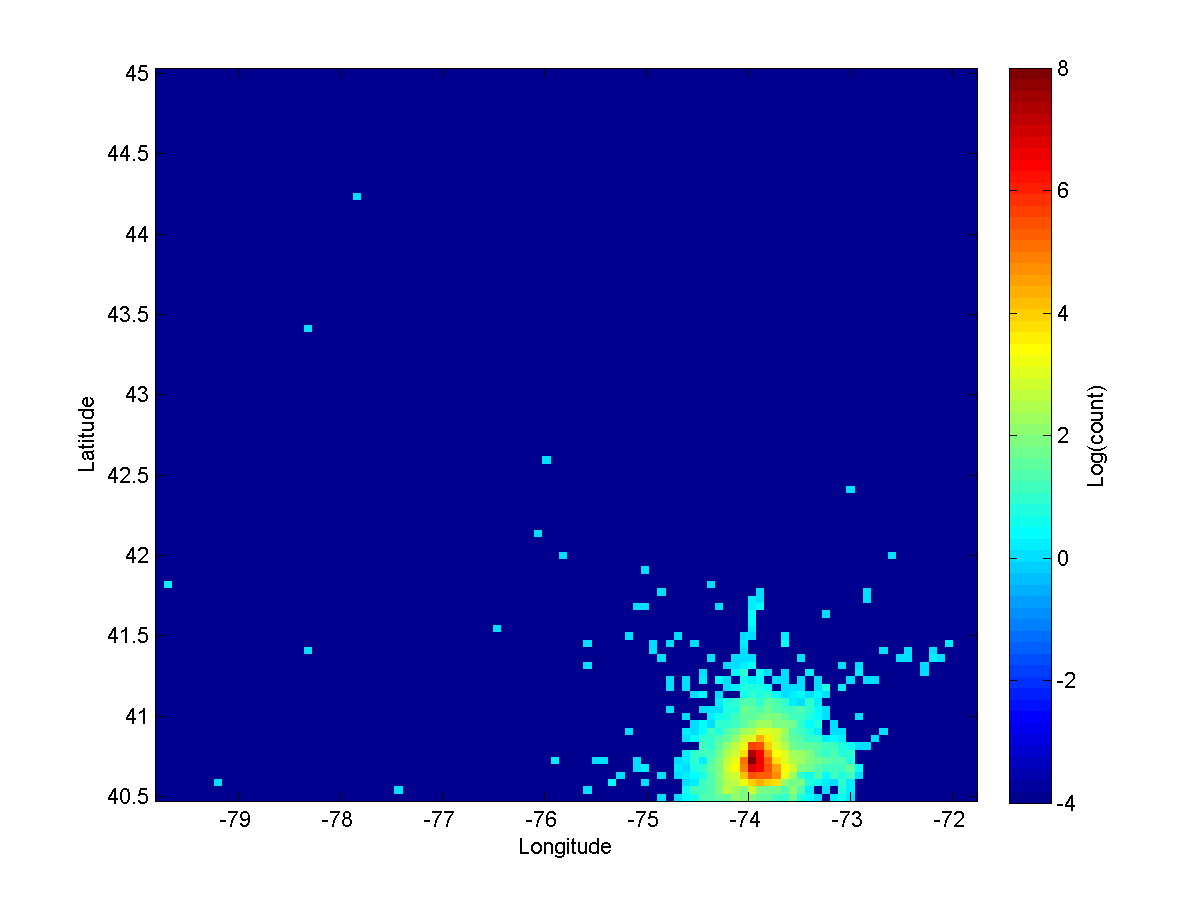
\includegraphics[scale=0.35]{dgrid.eps}
\caption{Density of taxi rides based on latitude and longitude.  The red section represents the location of the most rides, which is, unsurprisingly, located over the coordinates that correspond to Manhattan.}
\end{figure}

Day of week is an integer variable between 0 and 6 with Monday as the first day of the week, day 0. Time of day is a non-negative integer representing the time of day in seconds (0-86400). This represents every possible hour-minute-second combination for a given day. This is also an integer value. All distances are in miles. Start and end longitude and latitude are as standard GPS coordinates. These features are normalized to have a 0 mean and a standard deviation of 1 using the mean and standard deviation of all taxi data training examples. The output of this model is time in seconds the trip took rounded to a non-negative integer value.

\subsection{Training the Model}

For the purposes of this project, the data used is a sample of the larger data set. In this particular case the model is trained with 50,000 examples randomly selected from the larger data file of 173,000,000 examples. After the model was trained it was cross-validated on a set of 10,000 examples also randomly selected from the consolidated data file. From this cross-validation, the model was decided to be minimally regularized ($\lambda \approx 0.1$) and only have a polynomial regression up to $9^{th}$ terms.

Early in the development process, 1,000,000 training examples were used. However after comparing the runs from 1,000,000 examples and 30,000 examples (as can be seen in Figure 2 and Figure 3), along with a small sub-set learning curve, it was determined that minimal improvement was gained from using more than 50,000 examples. For this reason, and for testing and speed purposes, the smaller number was used.

\begin{figure}
\centering
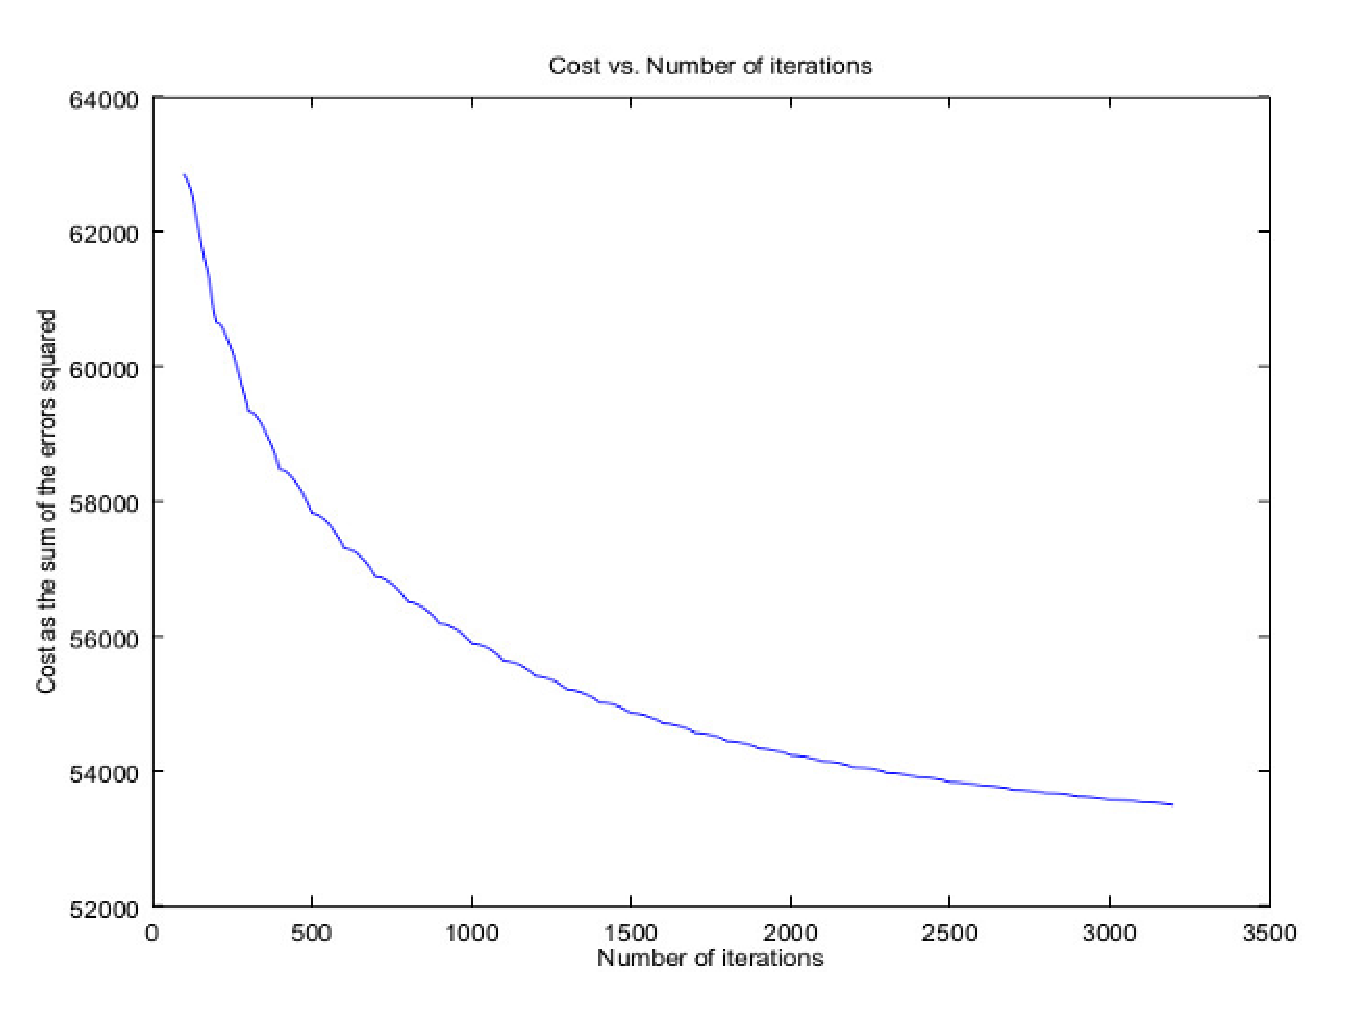
\includegraphics[scale=0.35]{Cost_Function_Graph_30k.eps}
\caption{Cost function vs. No. Iterations for 30k training examples}
\end{figure}
	
The current training method for the optimization problem is the fletcher-reeves form of conjugate gradient descent using a training step of .1 and running for about 3000 iterations. This gets a decent approximation of the prediction model's parameters. The model was cross-validated against a set of 10,000 training examples. The output of the training and cross-validation data is displayed as the average error measured in minutes. Using cross-validation the model parameters were varied until a good approximation was generated. Afterwards, the prediction parameters were tested against another set of 10,000 test examples to check for the model's ability to generalize. 

The model is trained separately from the rest of the program. This script is run either on the server, or off-site and the calculated values are exported to the server. The predictive model can then be used with a simple vector inner product calculation between the input and the calculated theta server side to generate the predicted time.

\begin{figure}
\centering
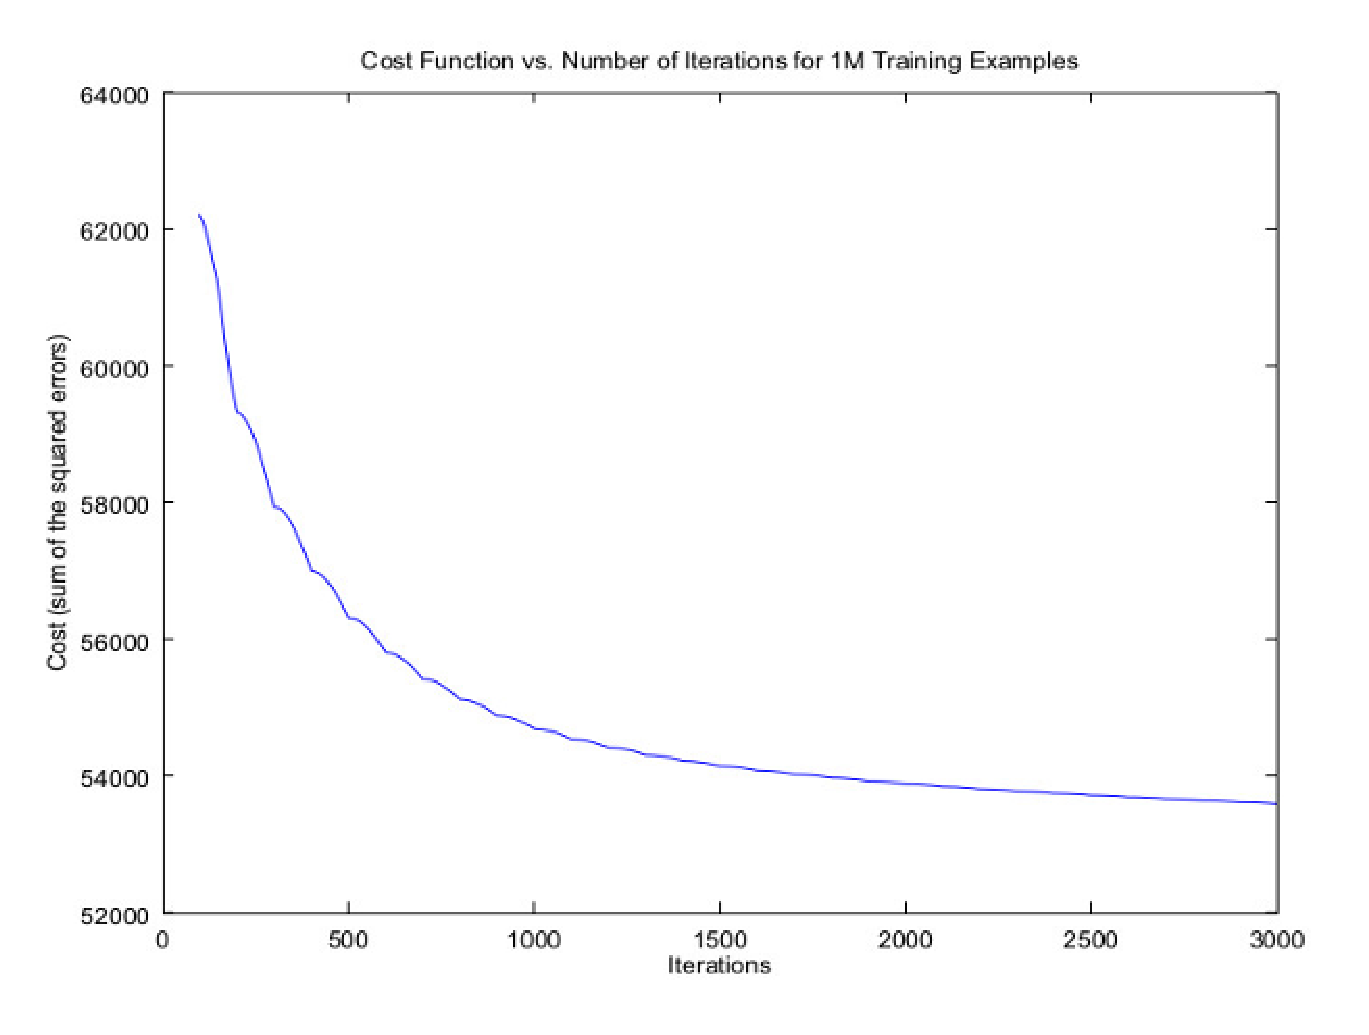
\includegraphics[scale=0.35]{Cost_Function_Graph_1M.eps}
\caption{Cost function vs. No. Iterations for 1 Million training examples}
\end{figure}

\subsection{The Model in Production}
	
If this were an ongoing project, it may be beneficial to rerun the training every 5,000,000 new examples saved from current Taxi Data or even once a month. Since the data covers an entire year, it's unlikely that the program needs to be run often. This is beneficial since with a large number of training examples, the model could take days to generate the best prediction possible. However, due to the historical nature of the data being used (Taxi Data from 2013), and the context of this project, it makes more sense for this endeavor to calculate theta once on a subset of the data and use it as the prediction model.

\section{Traffic and Search}

\subsection{Optimal path}
In order to determine the optimal path from one location in Manhattan to another, we used A* search on a directed graph representing discrete points on streets in New York.  We used an adjacency list to hold the graph data.  
 
We used Java to implement the search algorithm and adjacency list.  The rationale for using Java was twofold.  Firstly, the student implementing this part is more comfortable with Java than other languages that could perform the same functions.  Secondly, because we plan to package the end product in an Android mobile application, using Java was a logical choice.  It makes it easier to perform any interfacing or communication that is necessary between backend and frontend code since Android uses Java.
 
        	We calculated the optimal distances between points in New York by implementing A* search in Java.  It took us multiple code revisions before we started getting output that made any sense given our dataset.  There were a few difficulties in implementing this search algorithm.  One was accurately calculating distance between two nodes.  Initially we used the Haversine function to do so, but that was too imprecise because it relies on a radius.  In this case, that radius is the radius of the Earth.  Without an extremely precise measurement of the radius of the Earth at the latitude of a given node, this method was not useful.  Ultimately the far simpler distance formula proved to be more precise, as added distance due to the curve of the Earth is negligible in the range that are using \– Manhattan.

        	 The next major problem with implementing the search was that all of our map data came as discrete nodes.  In order to find an optimal path between two random coordinates, we had to figure out how to take coordinates that did not correspond to any existing node in our map and connect them to the map.  This meant checking the map for the node with coordinates closest to the input coordinates, which in turn meant iterating through the nodes every time we wanted to run a new path search.  This node-fitting proved to be extremely costly in regards to efficiency, so much so that we had to adjust our technique simply in order to be able to process our data in a matter of days instead of months.  We initially started including only nodes in range around Manhattan, which sped our search up considerably.  Ultimately, however, we subdivided our map into a grid, which we then used to search through possible nodes more quickly by eliminating large chunks of them at a time and only ever considering a small number of nodes.
%end

\subsection{Android application}
        	We have created an Android application that allows the user to enter coordinates for starting and ending locations in Manhattan and returns to the user the optimal distance and time.  In order to do this, we are housing our data on a server.  We are using AmazonWebServices to run a server application in the cloud, which the Android application can then connect to using a simple TCP socket in order to send and receive information.  The client application sends the coordinates to the server, which runs A* search to find the optimal distance and runs the calculations required to determine optimal time, which it then returns to the user.

\subsection{Overcharge statistics}
Analysis of the taxi data was ultimately performed in Java instead of Perl as Perl's IO read speed was substantially slower than that of Java's BufferedReader, taking over 10x as long to iterate through the same 100 million lines. Even so, Java still took around an hour to generate the data for the histograms, traffic movie, and overcharge statistics. The actual plots were made in matlab.

\section{Results}

\subsection{Map Data}
The road map was stored as a tsv. A modified version of ignacioarnaldo's Java application (MIT license) was used to generate this map. The procedure involved converting road way points to nodes and edges on a sparse graph. The reason that graph was made sparse is that many roads are not perfectly straight and consequently need multiple points to maintain the geometry. The final graph contained 1133702 nodes and 1254964 edges, of which 259464 were one-way and the rest bidirectional. The sparse nature of the graph is why an adjacency list representation was used for the A* search instead of an adjacency matrix.

\begin{figure}
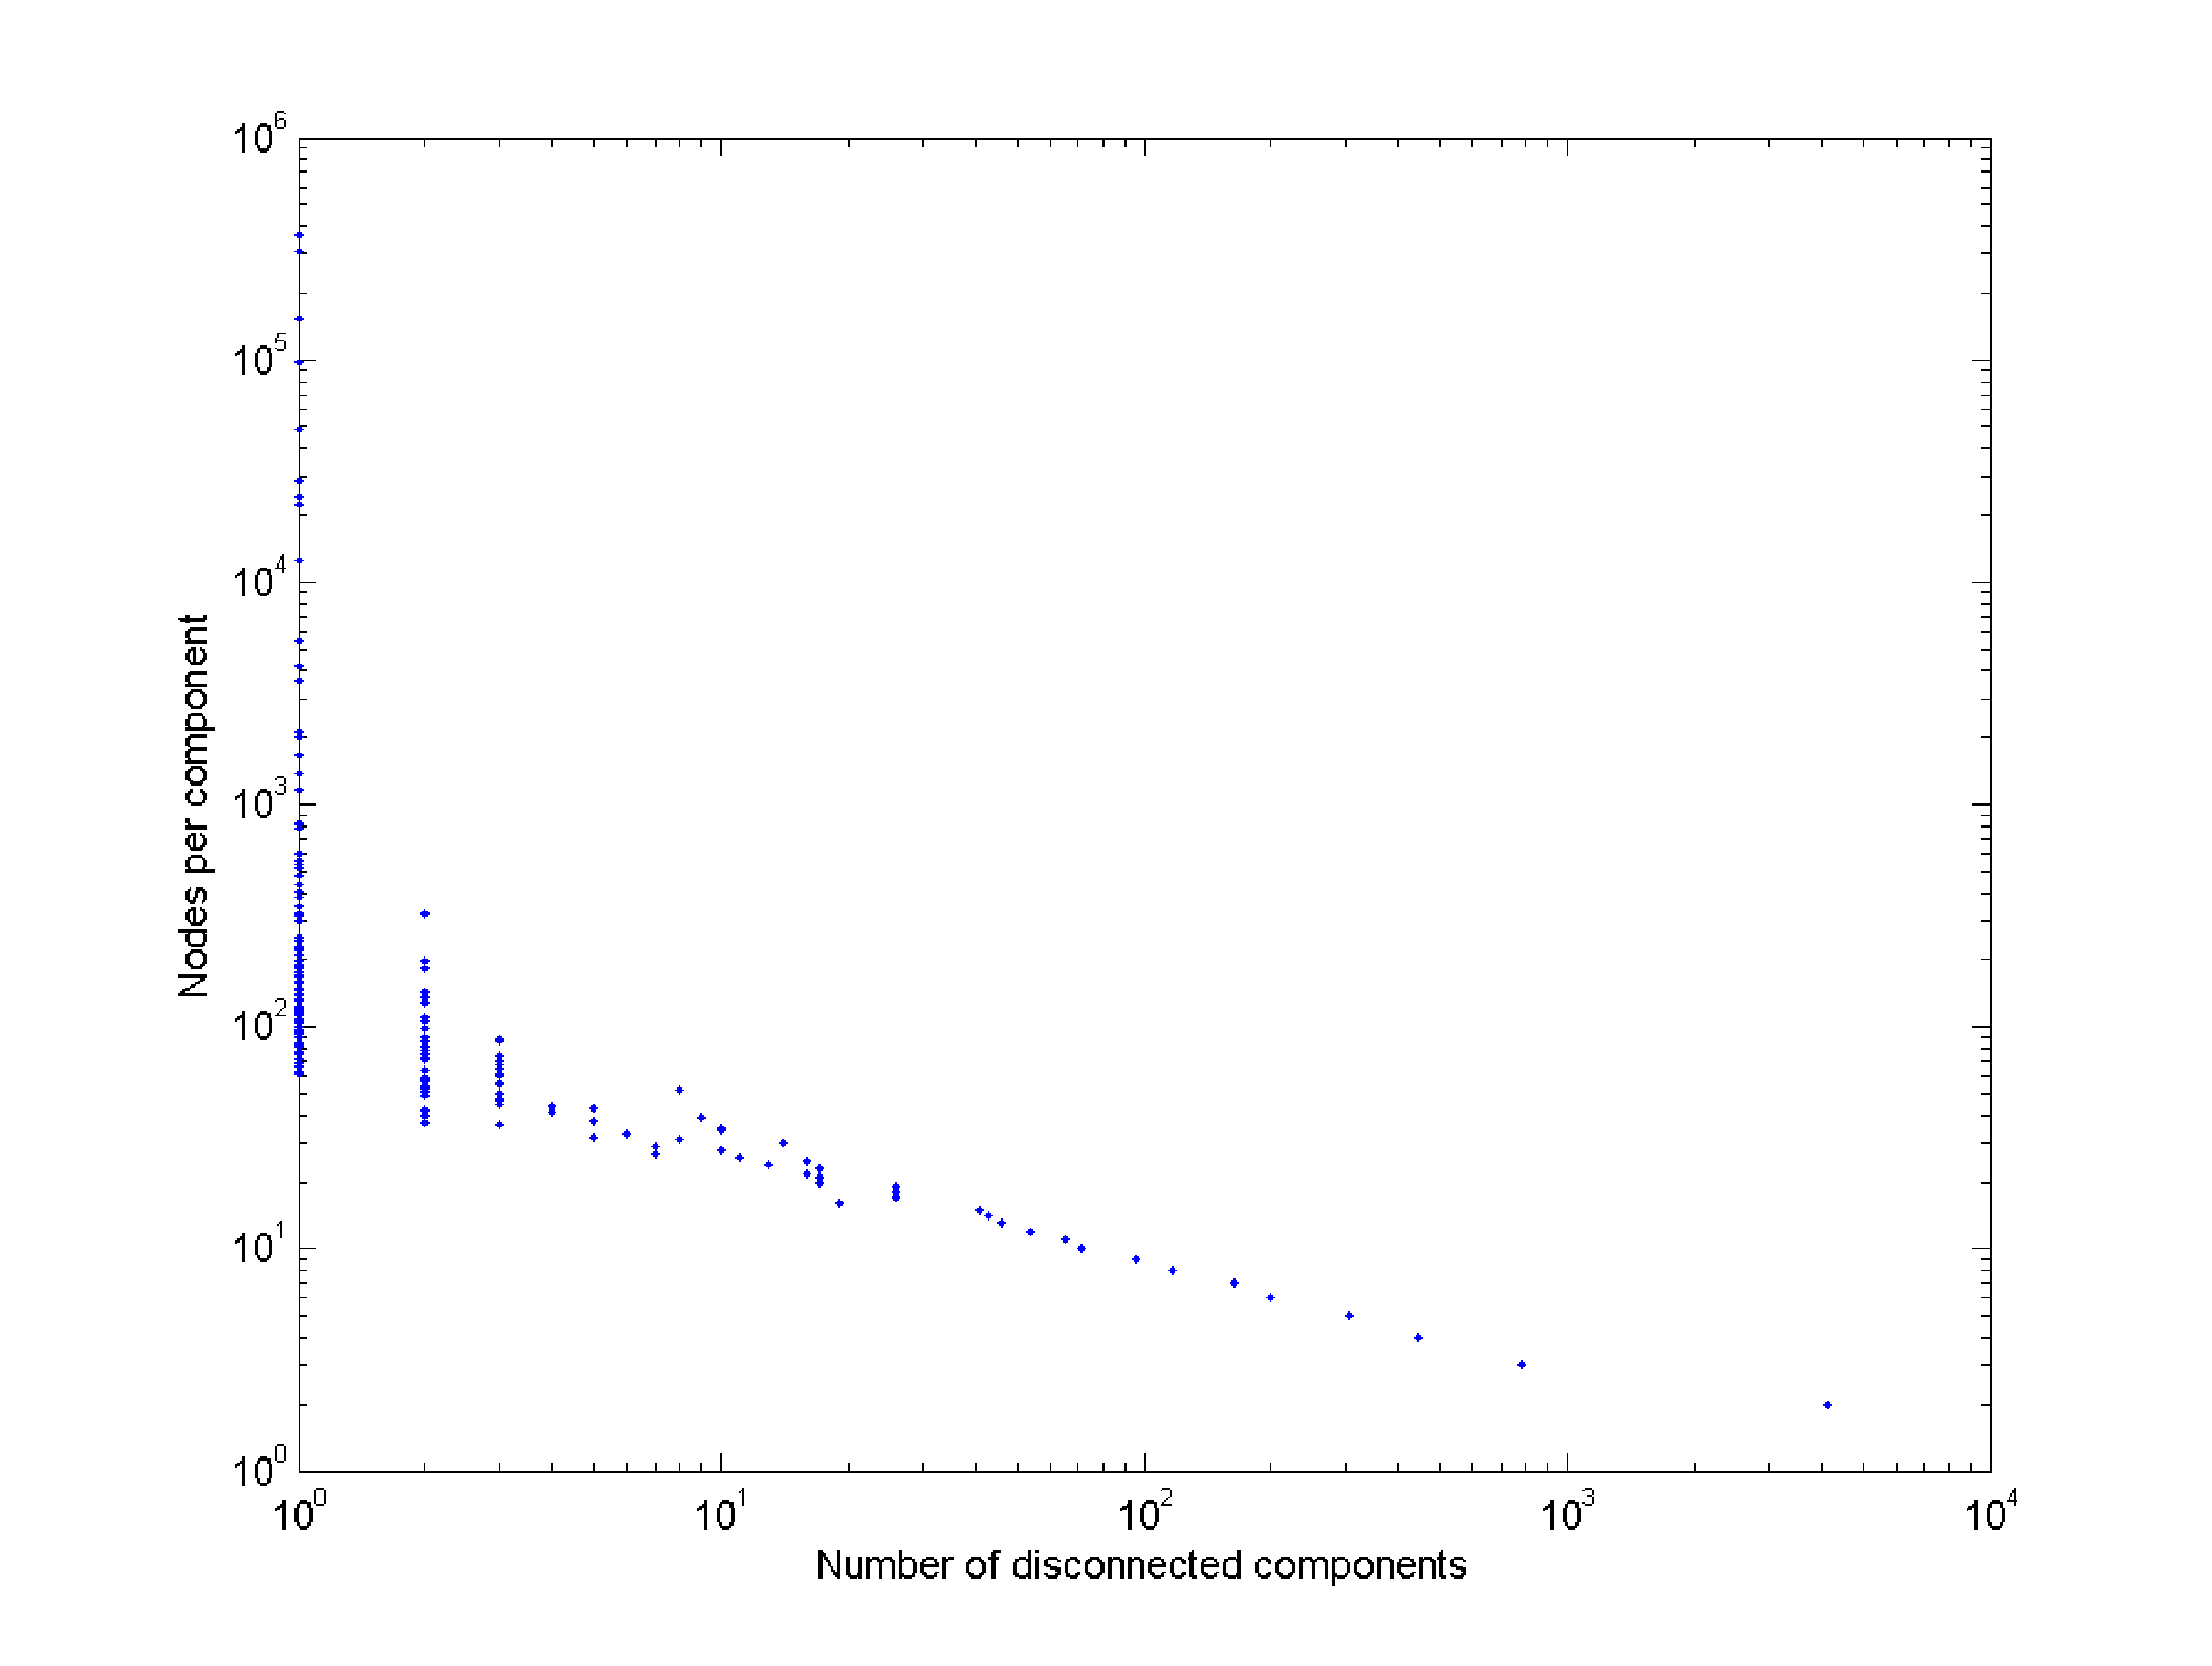
\includegraphics[scale=.20]{components.eps}
\caption{Distribution of graph components}
\end{figure}

\begin{figure}
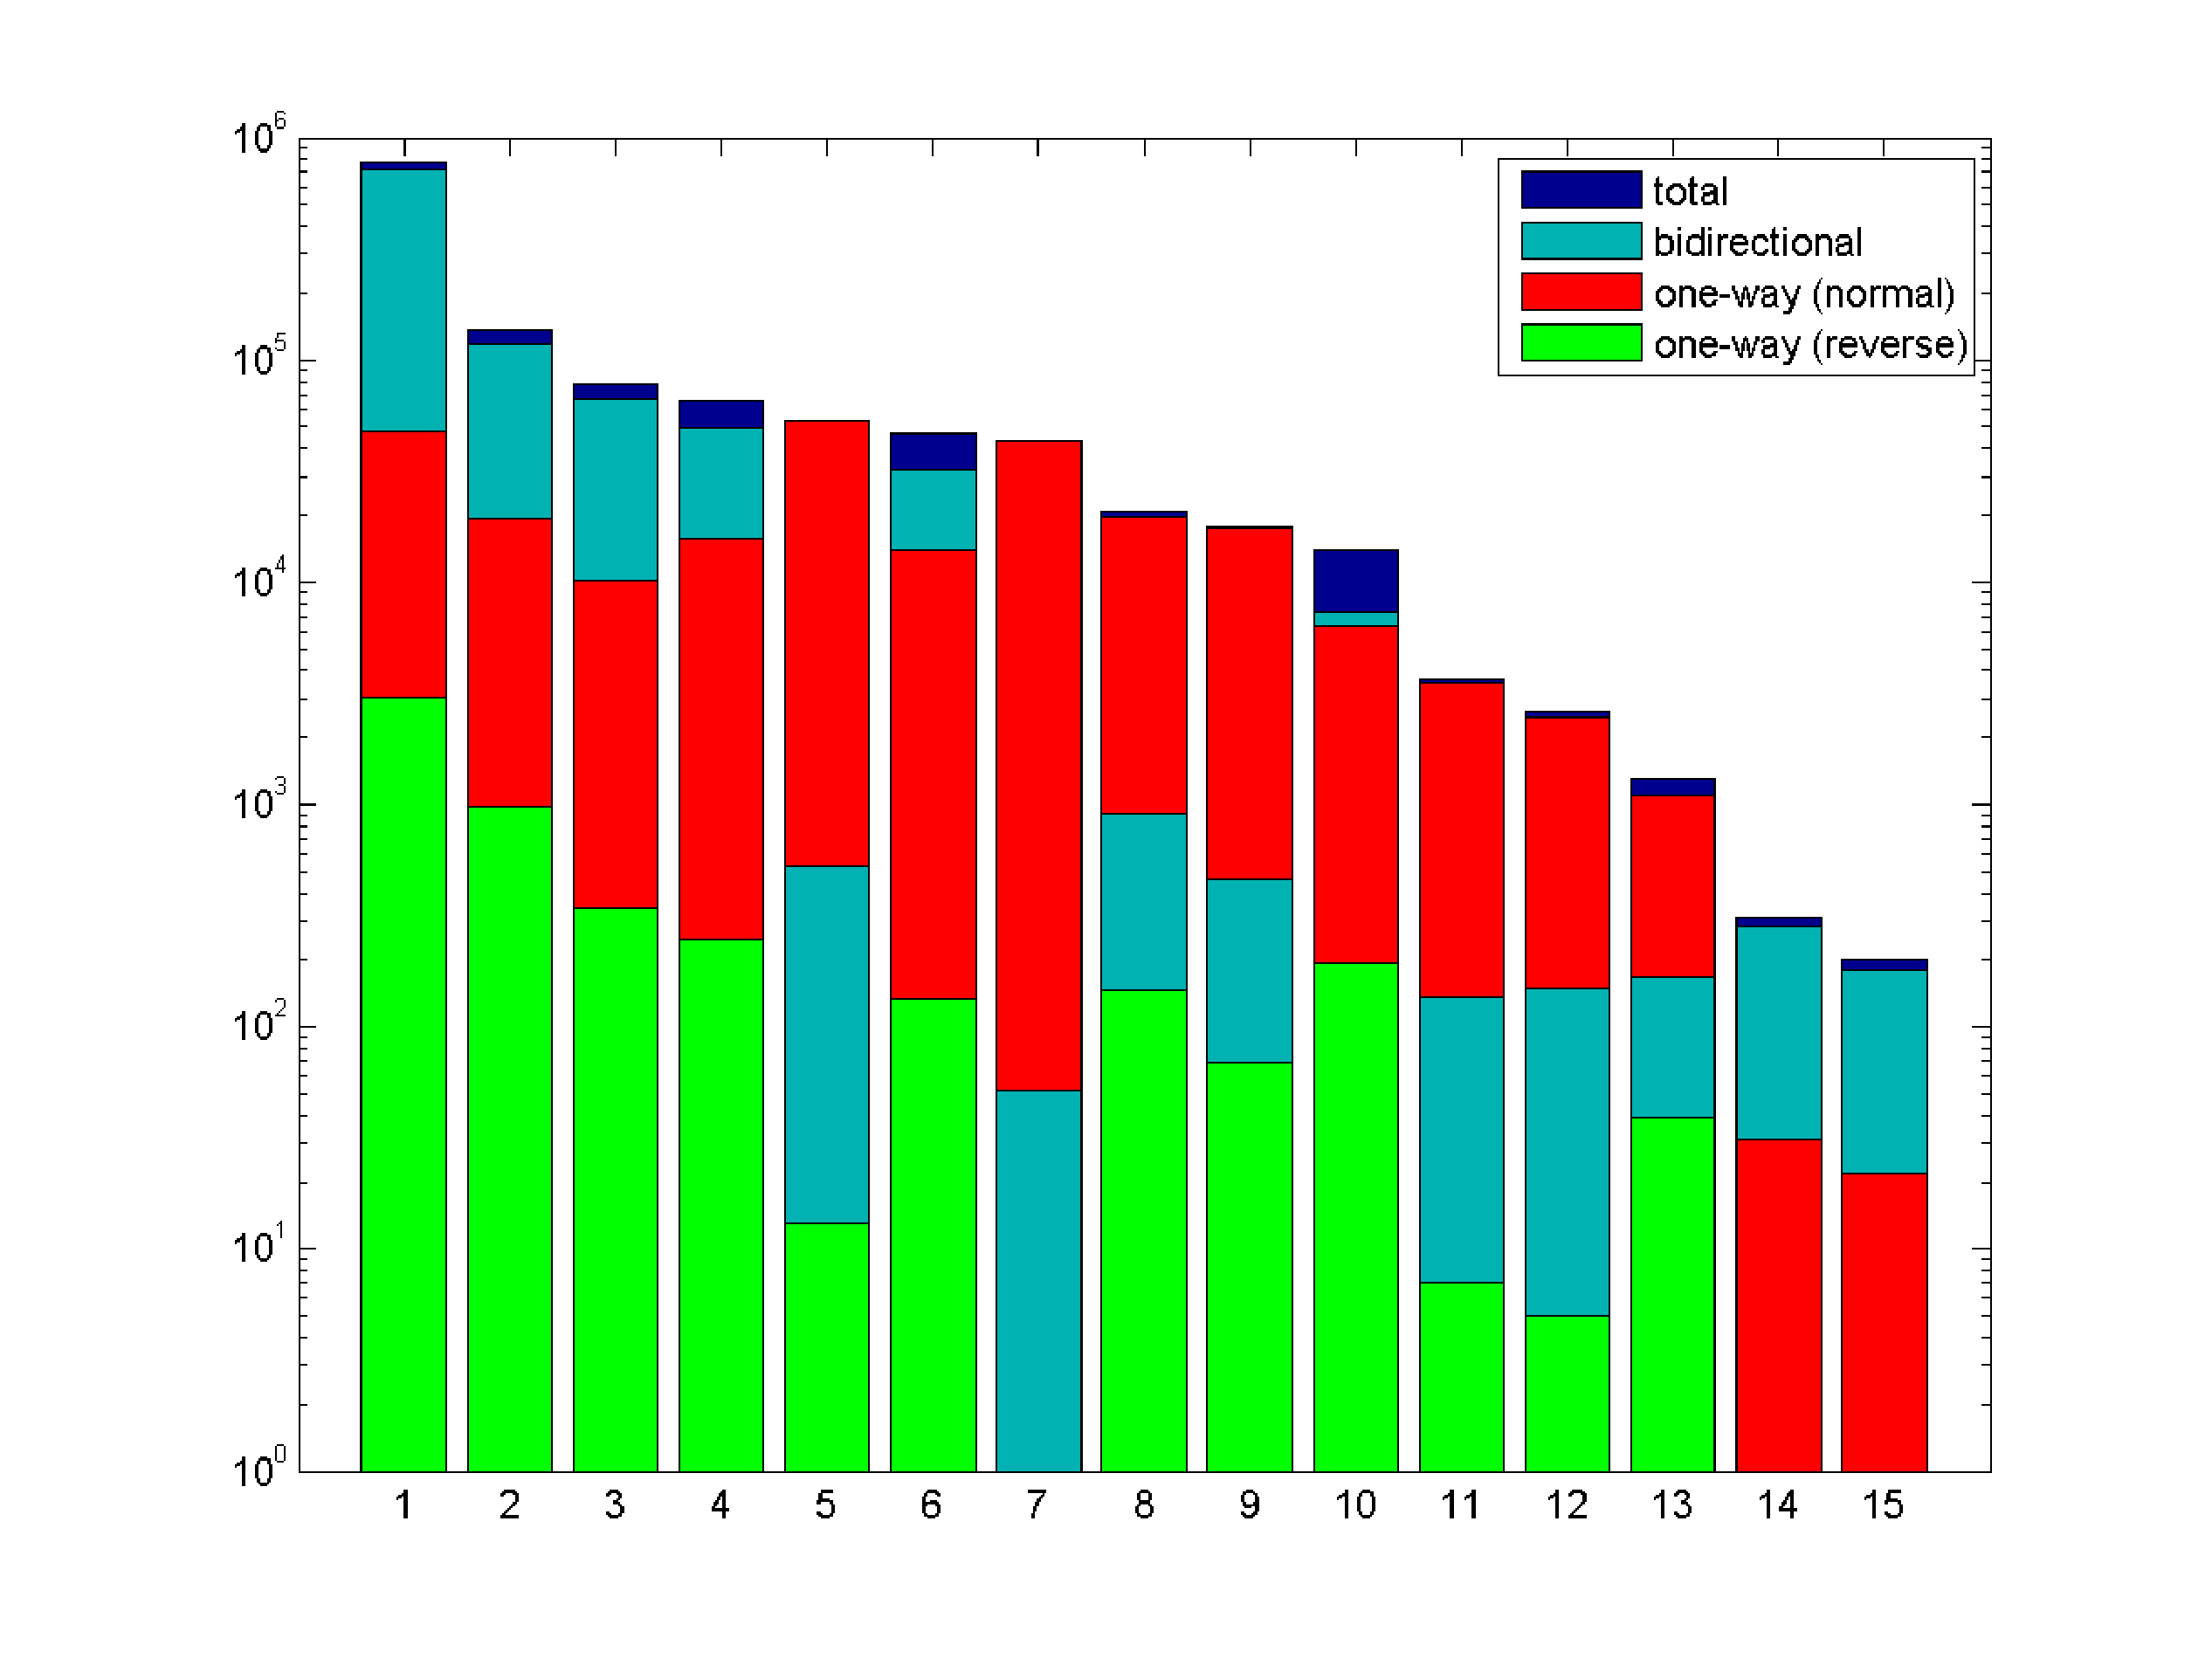
\includegraphics[scale=.20]{roads.eps}
\caption{Bar chart of the frequencies of the various road types. From left to right: residential roads, service roads, tertiary roads, secondary roads, motorway links, primary roads, motorways (freeways), truck roads, truck links, unclassified (minor) roads, primary links, secondary links, tertiary links, undetermined roads, and living streets.}
\end{figure}

The Open Street Map road feature set (retrieved in GEOJSON format from mapzen) contained two main types of roads (called highways in Open Street Map lingo). First, non-motor vehicle roads such as bridleways, footways, and paths (these all have specific definitions that can be found on the Open Street Map wiki). Second, motor vehicle roads such as  primary highways, residential roads, etc. Counts for the different motor-vehicle roads of interest are present in chart 1. Although the frequency of these types of roads did vary between weakly-connected components, the variance appeared fairly random. The frequency of types of roads does not differ from expectations - residential roads outnumber highways, and so forth.

Preliminary analysis of the graph (of New York, New York) from Open Street Map revealed the existence of 7049 disconnected components. Of these components, the existence of 4119 disconnected 2-node road segments is particularly noteworthy (Figure 4, scatter plot). These segments likely correspond to duplications present post-TIGER import. This is a known issue with regards to the Open Street Map map data; however, the maps in this open-source project are updated periodically, so this might not be a problem for future researchers. Notwithstanding the duplicate roads, the existence of smaller road networks ranging from 3 to 1000 nodes is concerning. Even among the large road networks, there are disconnects - one large network contains 362,961 nodes while another contains 306,461 nodes. It is not impossible that New York contains two large road networks, perhaps geographically separated, that are disconnected from each other; however the fact that there are 7 other networks all containing over 10k nodes is highly implausible. A more likely conclusion is the Open Street Map data not only contains duplicate nodes, but also duplicate node networks. Nonetheless, with regards to accuracy, the road network duplication is not important, as nodes on different networks that result in the A* search failing were excluded from the overcharge analysis. The fragmented nature of the OSM data does explain why many of the A* searches were unable to find paths for corresponding taxi trips.

\subsection{A* Search}
Around a hundred million taxi rides were processed. The processing occurred on 12 cores, each core running through a single file of taxi data (12 files total), taking 48 hours total to process all the data. To speed up the time of the search, several improvements were made to a naive A* search. First, in addition to the heuristic of euclidean distance to destination, a second heuristic (taxi distance) was used to limit the distance of the path found to within .5 miles of that traveled by the taxi (Figure 14). Second, to find the start and end points from a given latitude and longitude, a 1000x1000 grid was created to cover the city. Each node was assigned to a square on this grid. This way, the start and end points could be looked up in the correspond square (along with surrounding squares, to account for, literally, "corner" cases), instead of needing to iterate through all the points. Together, these two improvements improved the speed of the search by a factor of 15. Each rectangle was 4.2 miles (longitude) by 3.12 miles (latitude). The distribution is shown in Figure 1.

When implementing A* search, we looked at the first 20 or so lines of historic taxi data to determine if A* was indeed outputting reasonable distances for trips.  By using latitude and longitude points on of actual trips and Google Maps, we were able to find out a few things about the data.

The entry for line 12 in trip\_data\_1, our first file of historic taxi data, has a distance of 1.3 miles.  Google Maps produced a similar estimate when we searched for a route using the same starting and ending points.  The distance we calculated using A*, however, was 1.8.  After looking at the map data, it appeared that the 65th Street Transverse through Central Park was not connected to any other roads on the map.  Knowing this, we went again to Google Maps and searched for the same trip, but adding a waypoint outside of Central Park, essentially forcing it to take a path that did not include the 65th Street Transverse. Google's optimal path without using the transverse came out to about 1.8 miles. The conclusion we drew from this was that our algorithm was correct, but that the map data is not completely accurate.  That conclusion should account for any A* estimations that are longer than the distance of the actual ride.  There were, however, still some trips that were inexplicably shorter than the estimated distance using A*.  Upon a closer look, we found that the trip data has distances in increments of tenths of a mile.  This made sense, as fares are calculated using tenths of a mile.  Some of the calculated distances were still longer, but when truncated to the tenths place were the same as the actual ride.
 
Looking at the first 20 or so lines of output, there was actually an example of a ride that was much longer than it should have been.  Line 14 of our data file has a ride distance of 2.3 miles, but the estimation was about 1.57 miles. After checking on Google Maps, the 1.57-mile estimate turned out to be accurate.  This was a good indication that the kind of overcharging that we hoped to find actually existed in some cases.


\begin{figure}
%\centering
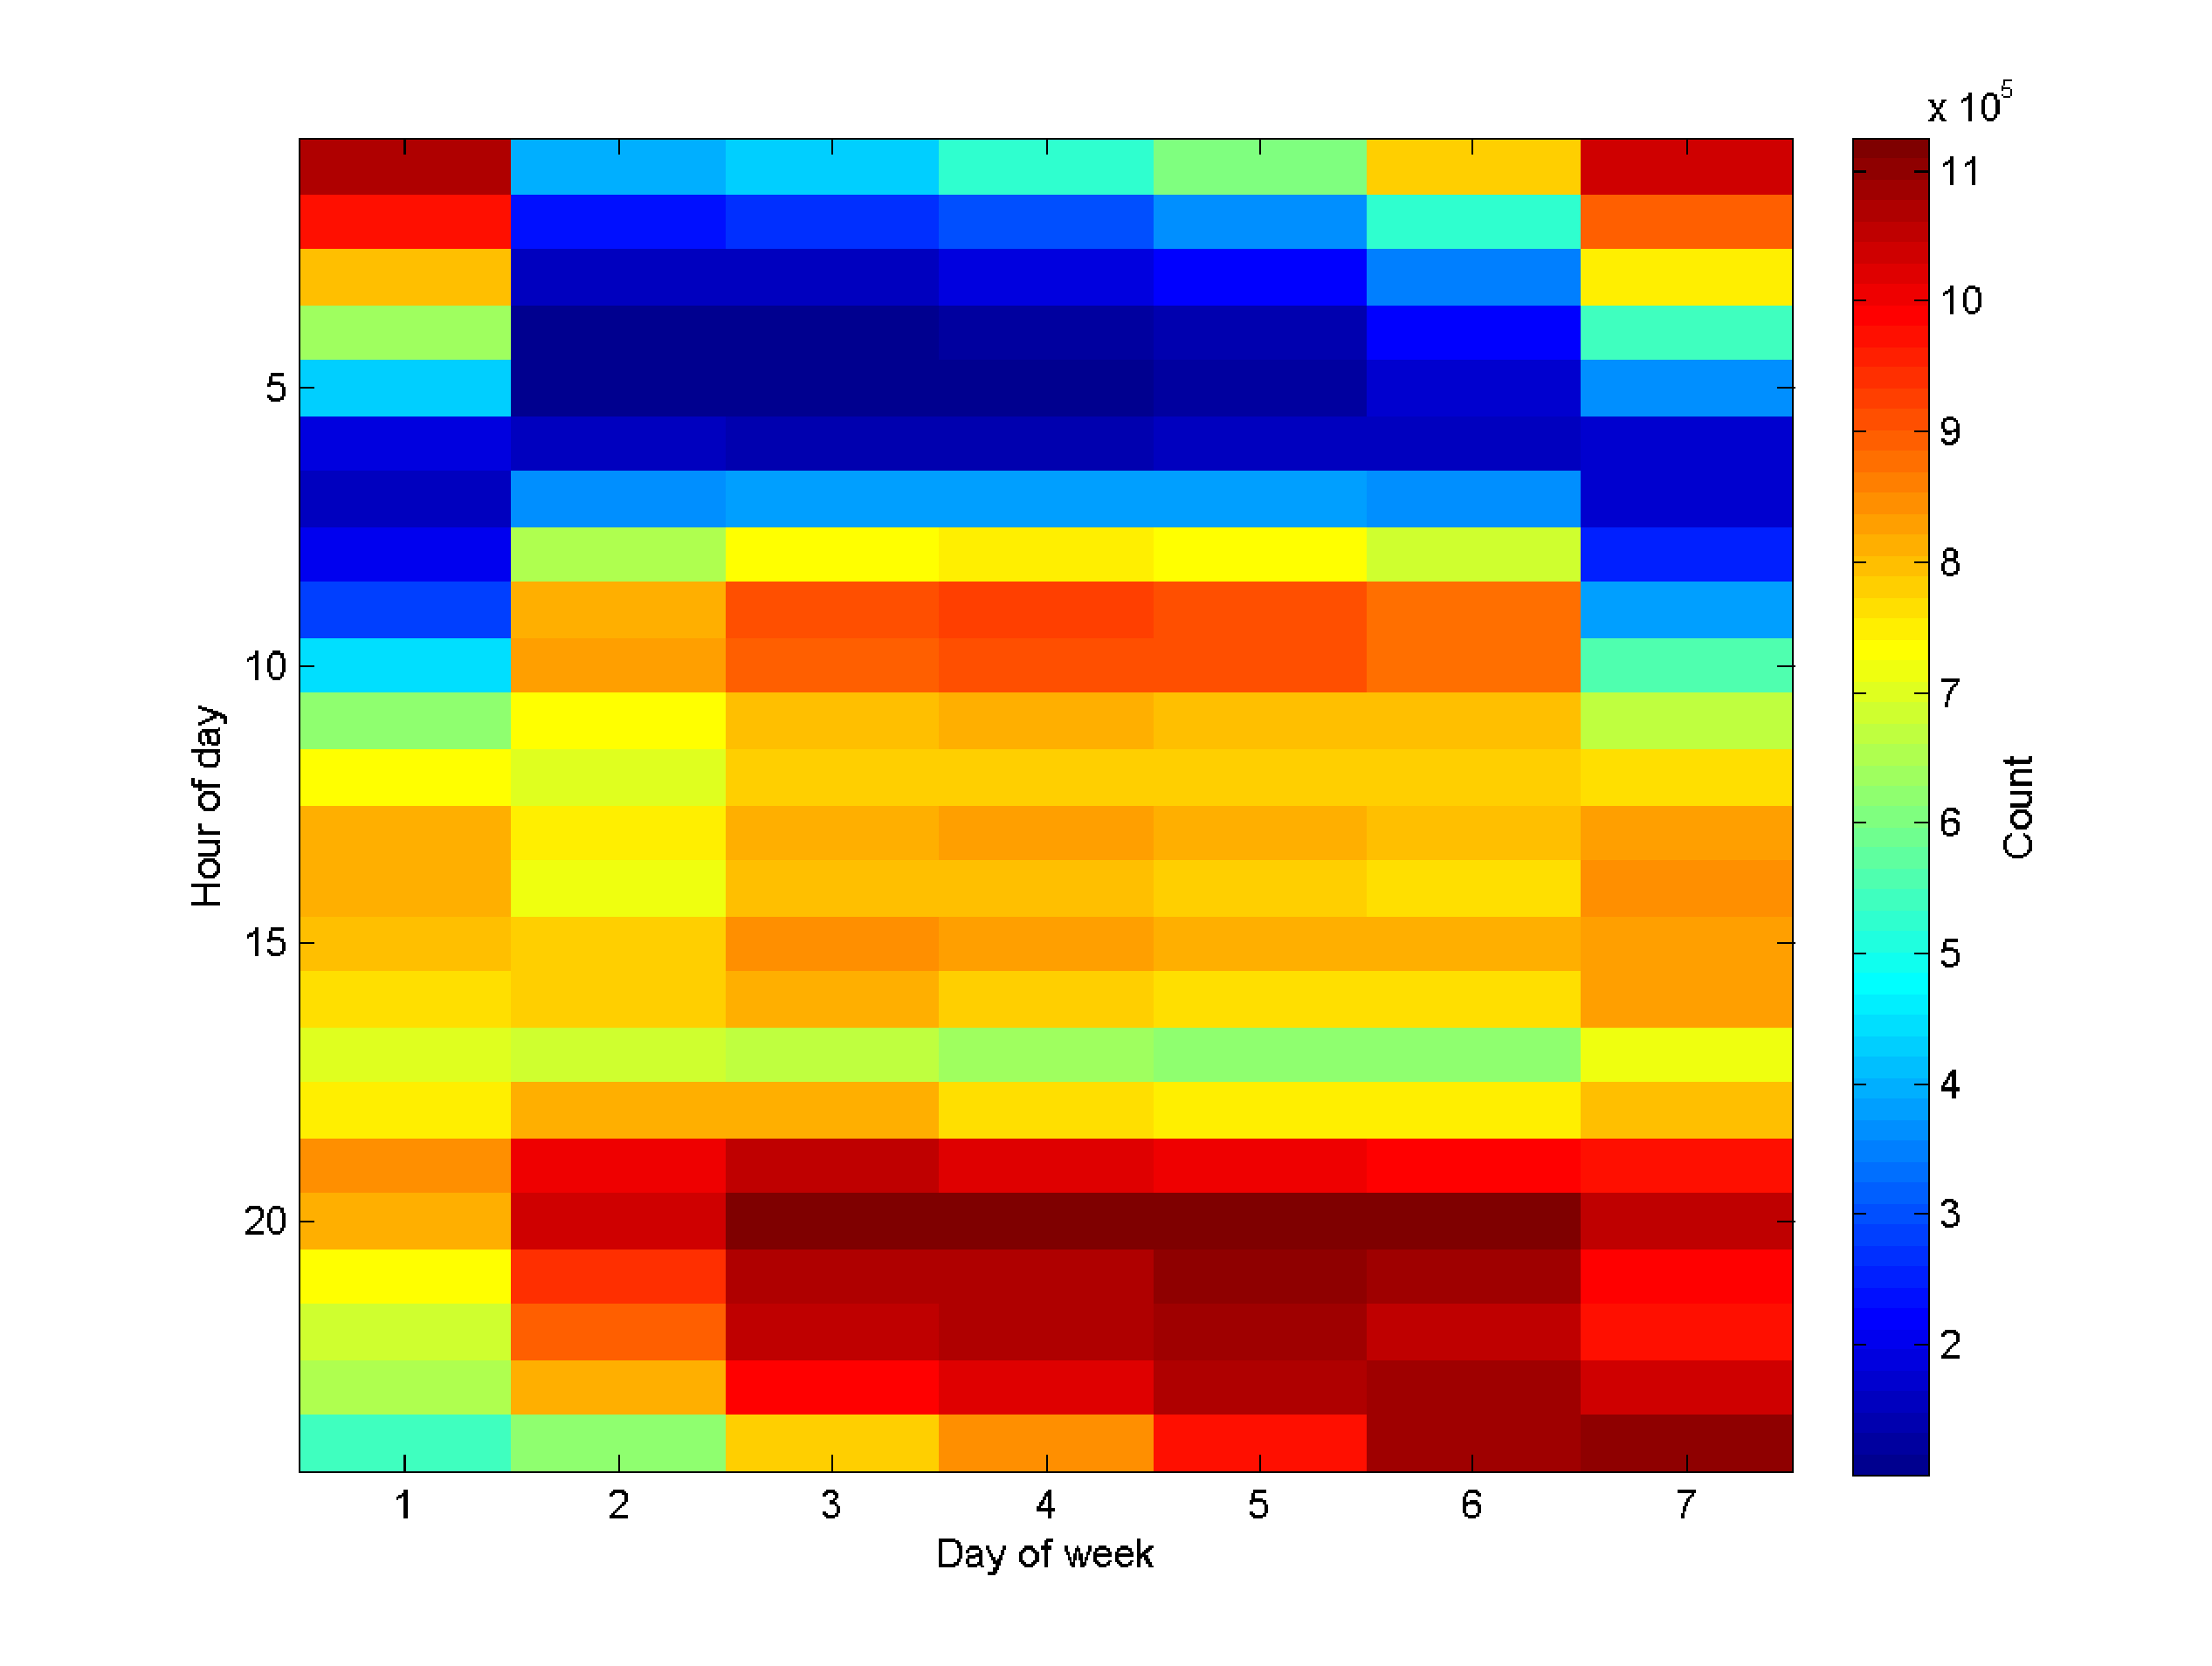
\includegraphics[scale=.20]{tgrid.eps}
\caption{Taxi distribution over time}
\end{figure}

\begin{figure}
%\centering
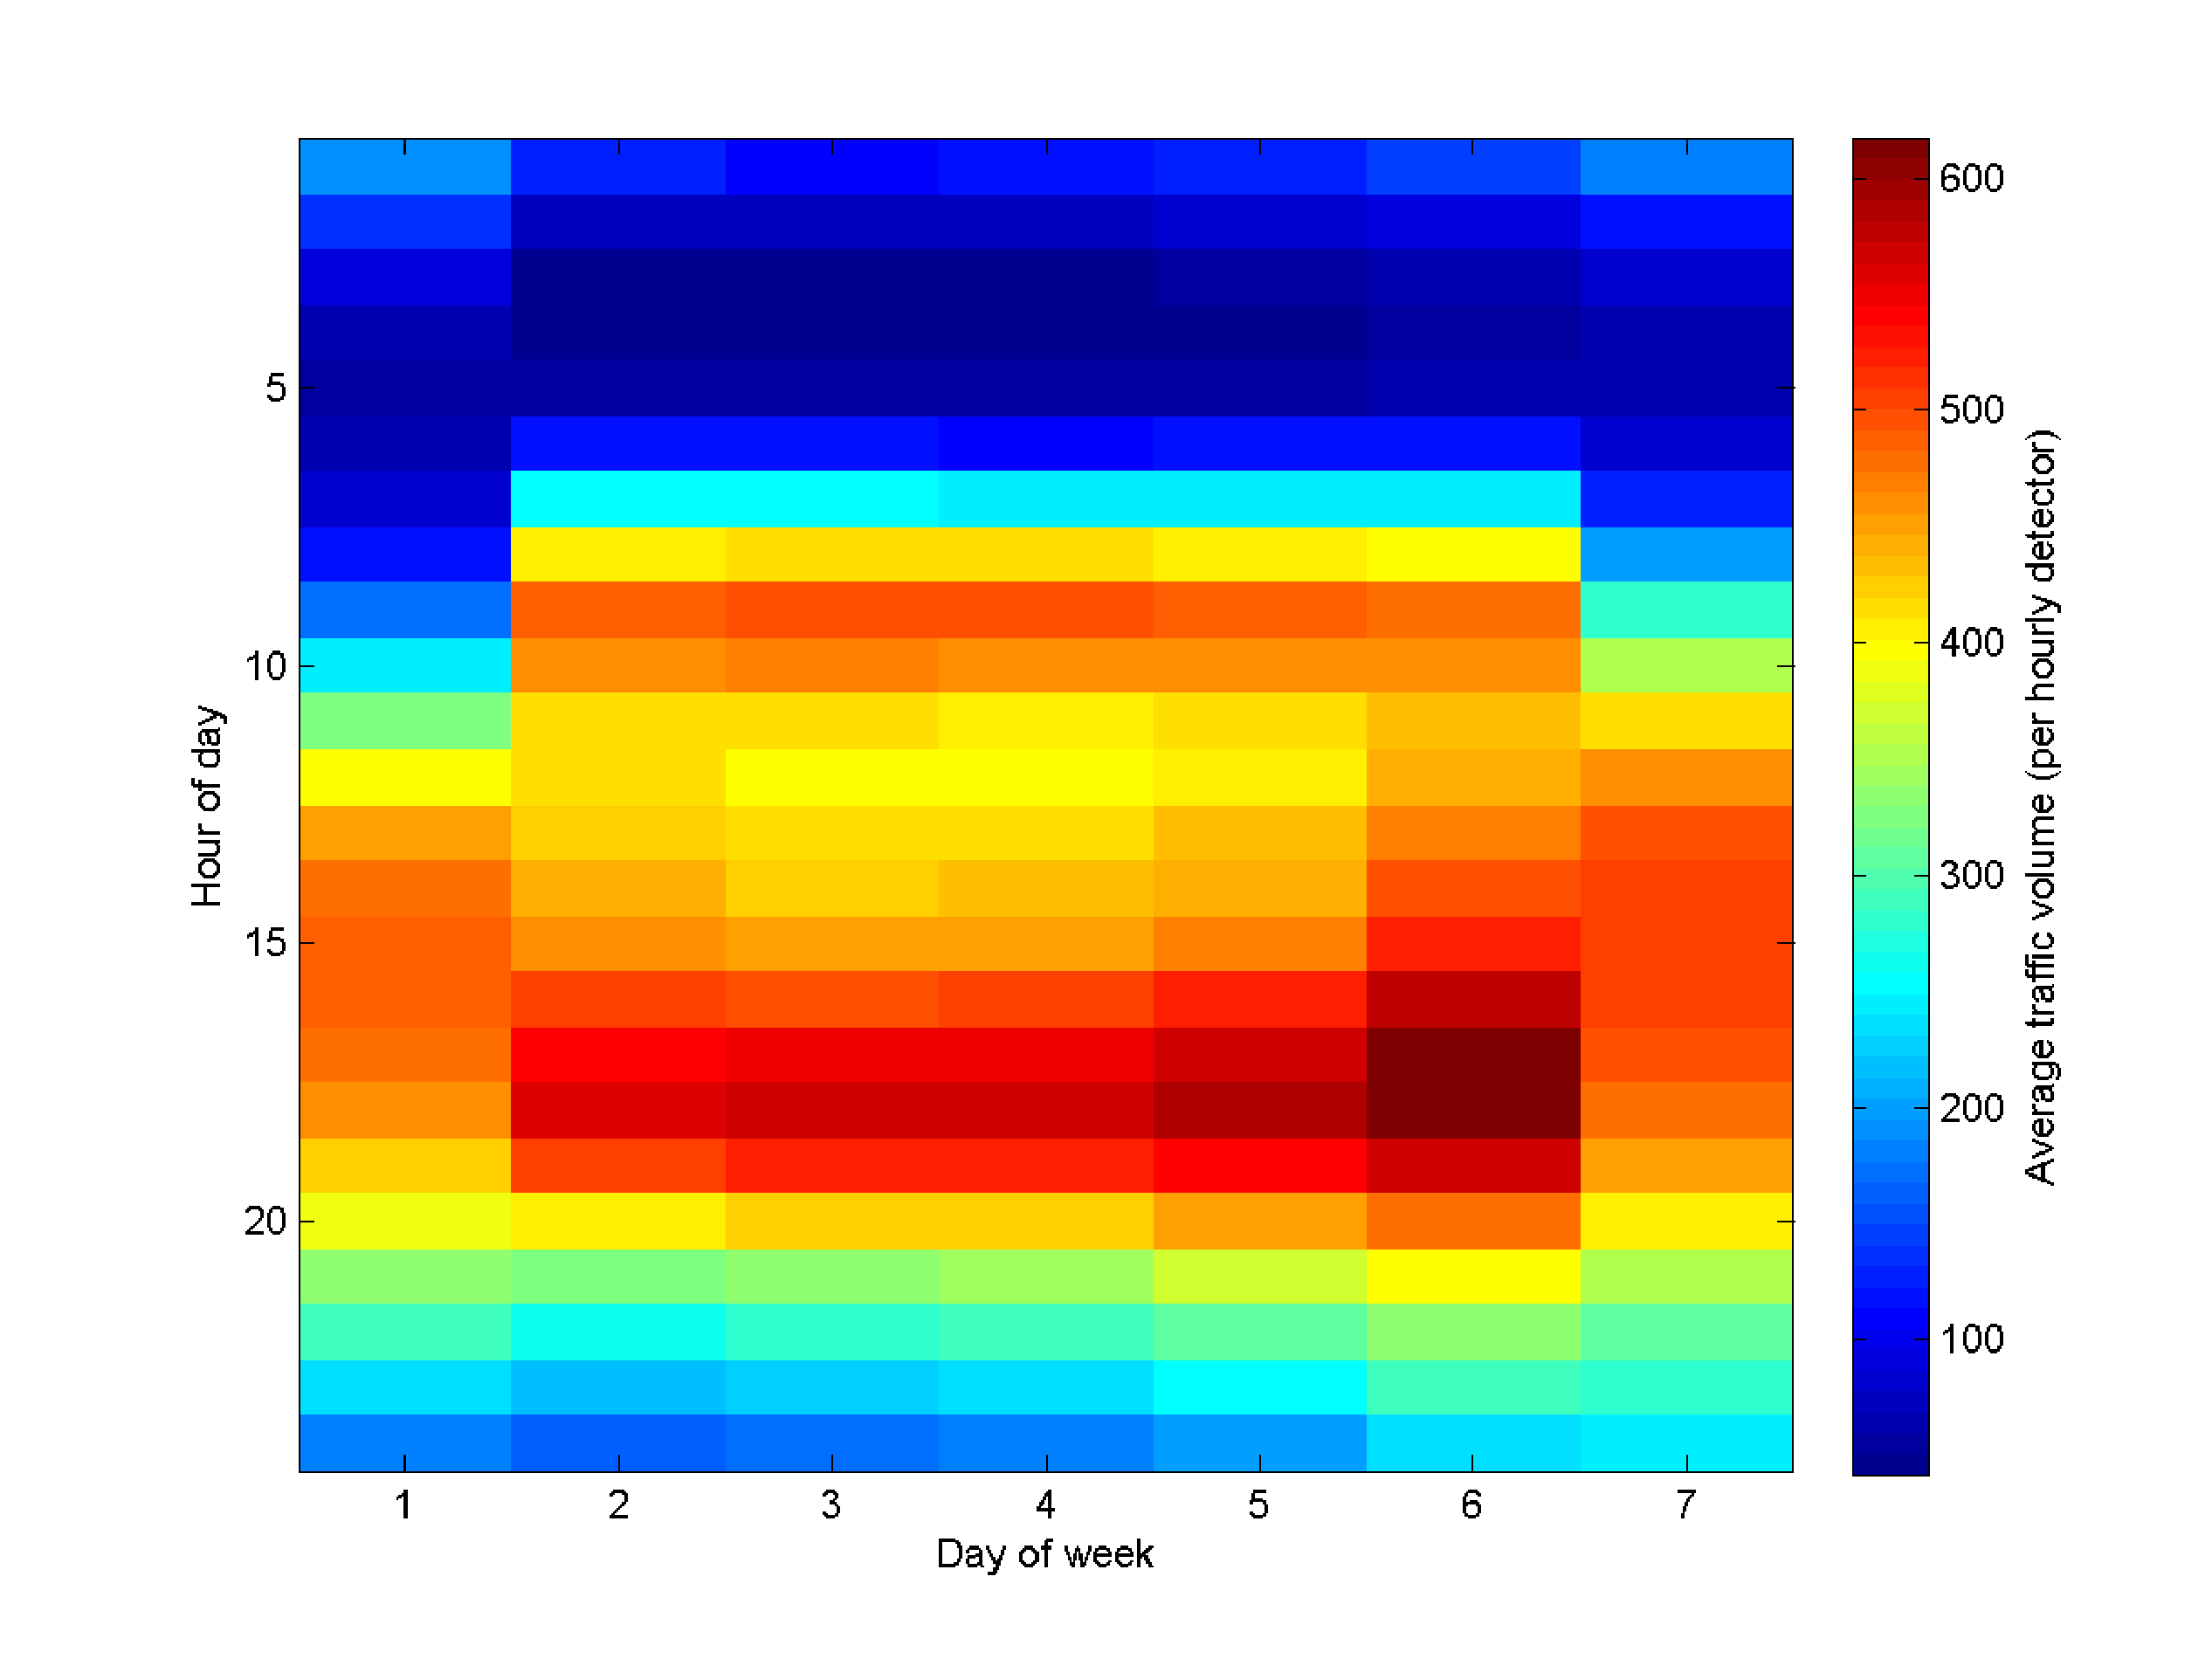
\includegraphics[scale=.20]{trgrid.eps}
\caption{Traffic volume}
\end{figure}

\subsection{Historic Taxi Data}

Preliminary analysis of the taxi data revealed that only 56.57\% of trips were valid; of these, only 81.86\% could be used for the overcharge analysis, as the A* search was unable to find valid paths for the rest. The various errors, along with their associated frequencies, are described in figures 8, 9. The types of errors (duplications, typos, mismatching duration and start/end time, trips lasting several days, etc) suggest that the recording devices on the taxi's were often dysfunctional, perhaps due to calibration difficulties. Often times, a latitude or longitude over a hundred or less than 10 would be encountered, with the taxi trip spanning over a thousand geographic miles. Nonetheless, a reasonable distance would be specified in the data, suggesting a typo (typing the same number twice) or omission (skipping over a number) might be responsible for the abnormally large or small coordinate, respectively.

Taxi volume correlates fairly well with traffic counts (Figures 6, 7). The two do appear to be offset by a couple hours, however.

\subsection{Model Results and Overcharge}



As shown in Figure 11, the taxi trip geographic distribution is bimodal, with peaks around .7 and 11 miles. Based on this geographic distribution, the grid was subdivided into 100 squares for the traffic model, so that most trips would be contained within a single square spanning 13 square miles. The trip time appears to have a single, broad peak around 400 seconds (Figure 10). Interestingly enough, around 14 thousand times as many rides lasted for a whole number of minutes compared to those at any other second. That 99.29\% of rides lasted a whole number of minutes suggests that many taxis may still be using outdated equipment that records trip duration to the nearest minute instead of the nearest second.

Perhaps more interesting is the shape of the overcharge statistics. The curve exhibits exponential decay, suggesting the possibility of rare but substantial instances of overcharge (Figure 13).

One major problem with the overcharge statistics in their current iteration relates to distance overestimates or underestimates caused by the selection of the closest intersection to the given start latitude/longitude or destination latitude/longitude. While it is not necessarily an unreasonable assumption that many trips start and end near intersections, it does introduce the possibility for error. Figure 14 shows the distance distribution from start and end nodes (histogram), while figure 13 displays the overcharge distribution. Although the error resulting from the use of intersections does impact the accuracy of results, the much bigger loss of accuracy appears to be a consequence of the unreliable map data. This might not be as big of problem for future researchers, however, since Open Street Map is a work in progress that is improving over time.

\begin{figure}
%\centering
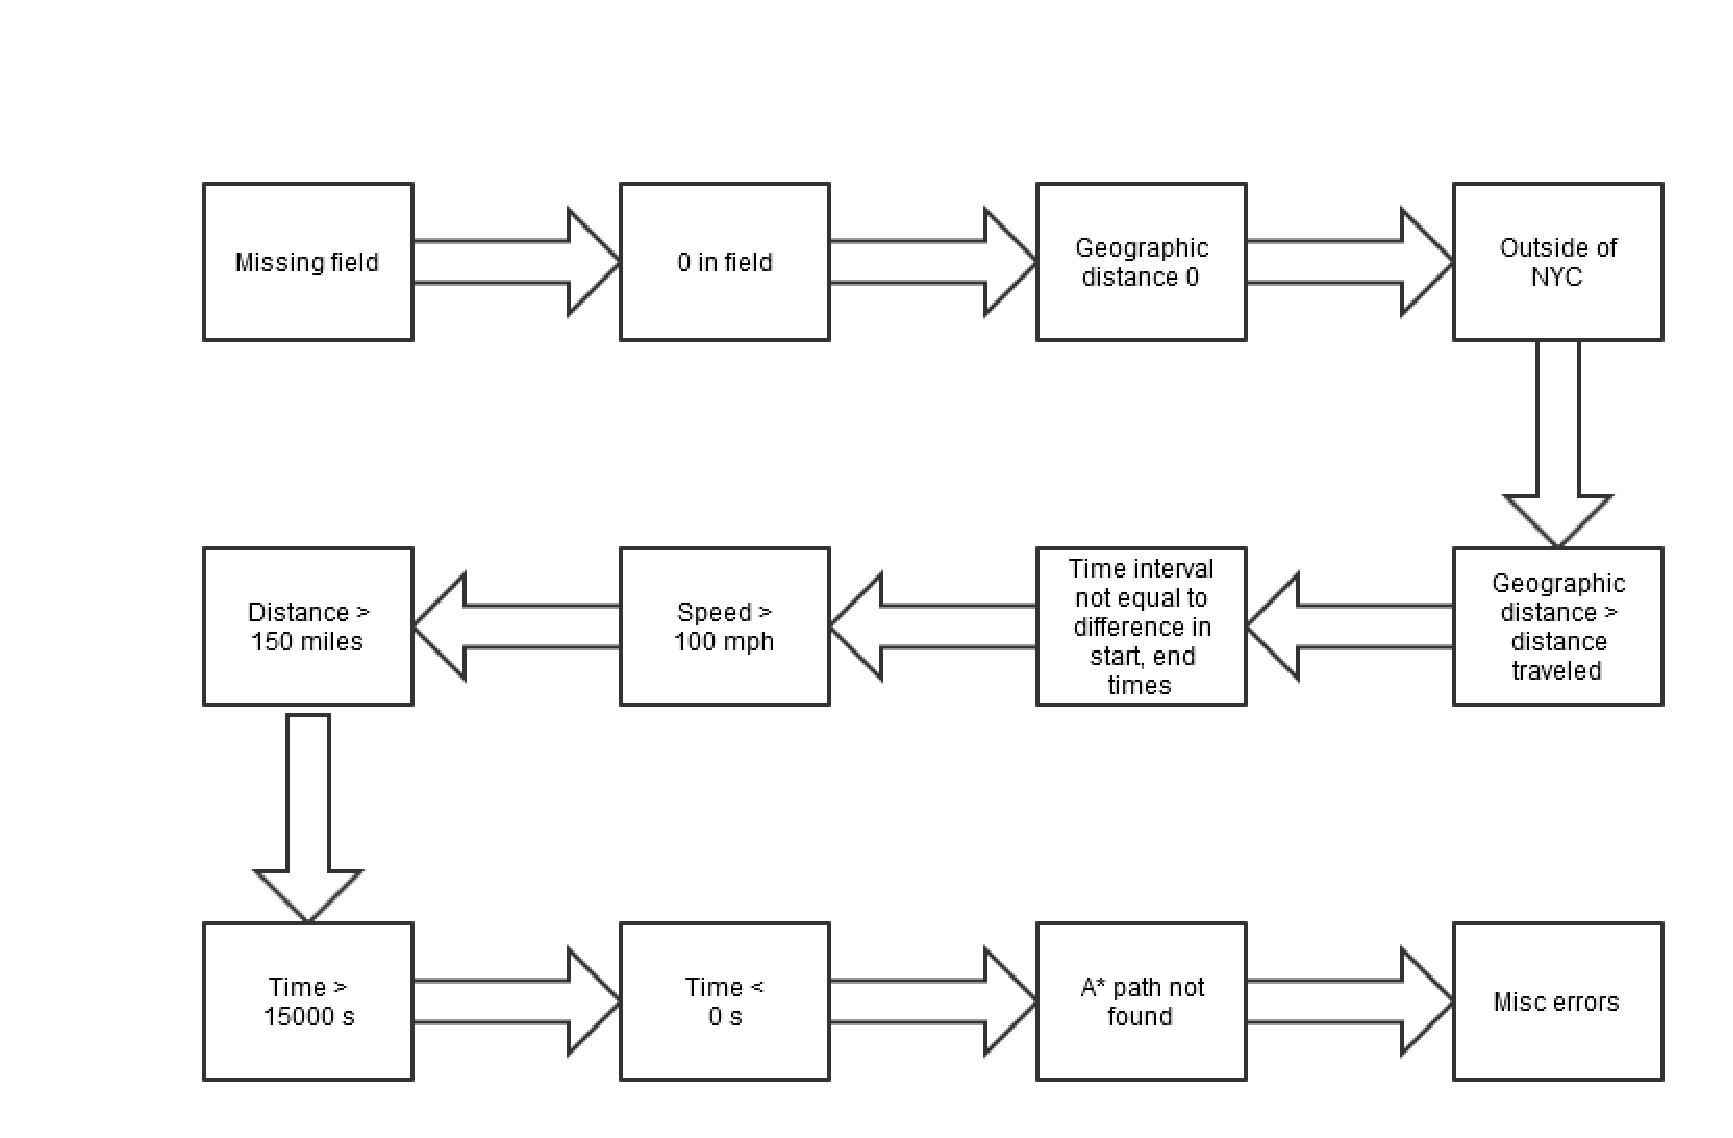
\includegraphics[scale=.25]{flow2.eps}
\caption{Flowchart of error pruning process}
\end{figure}

\begin{figure}
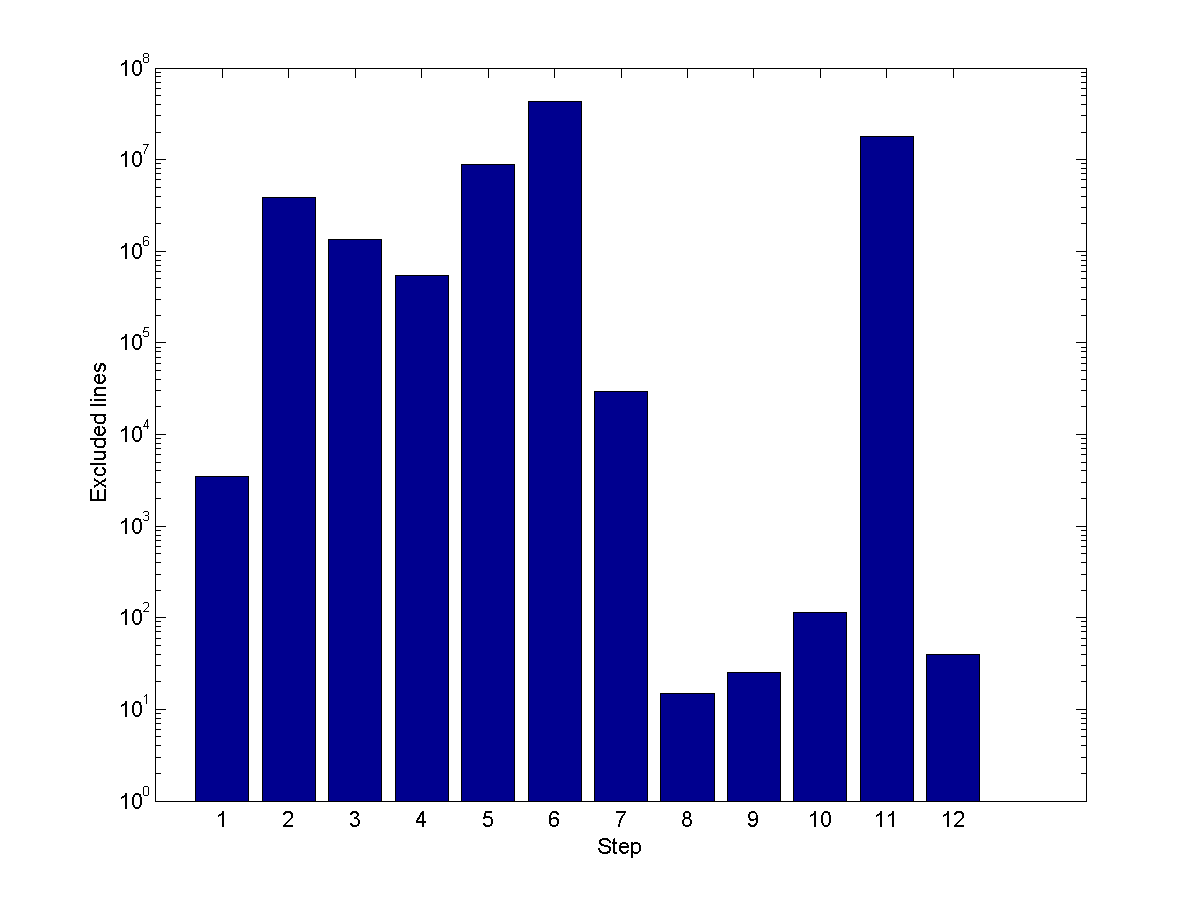
\includegraphics[scale=.35]{ebar.eps}
\caption{Number of lines excluded at each step of the pruning process}
\end{figure}

\begin{figure}
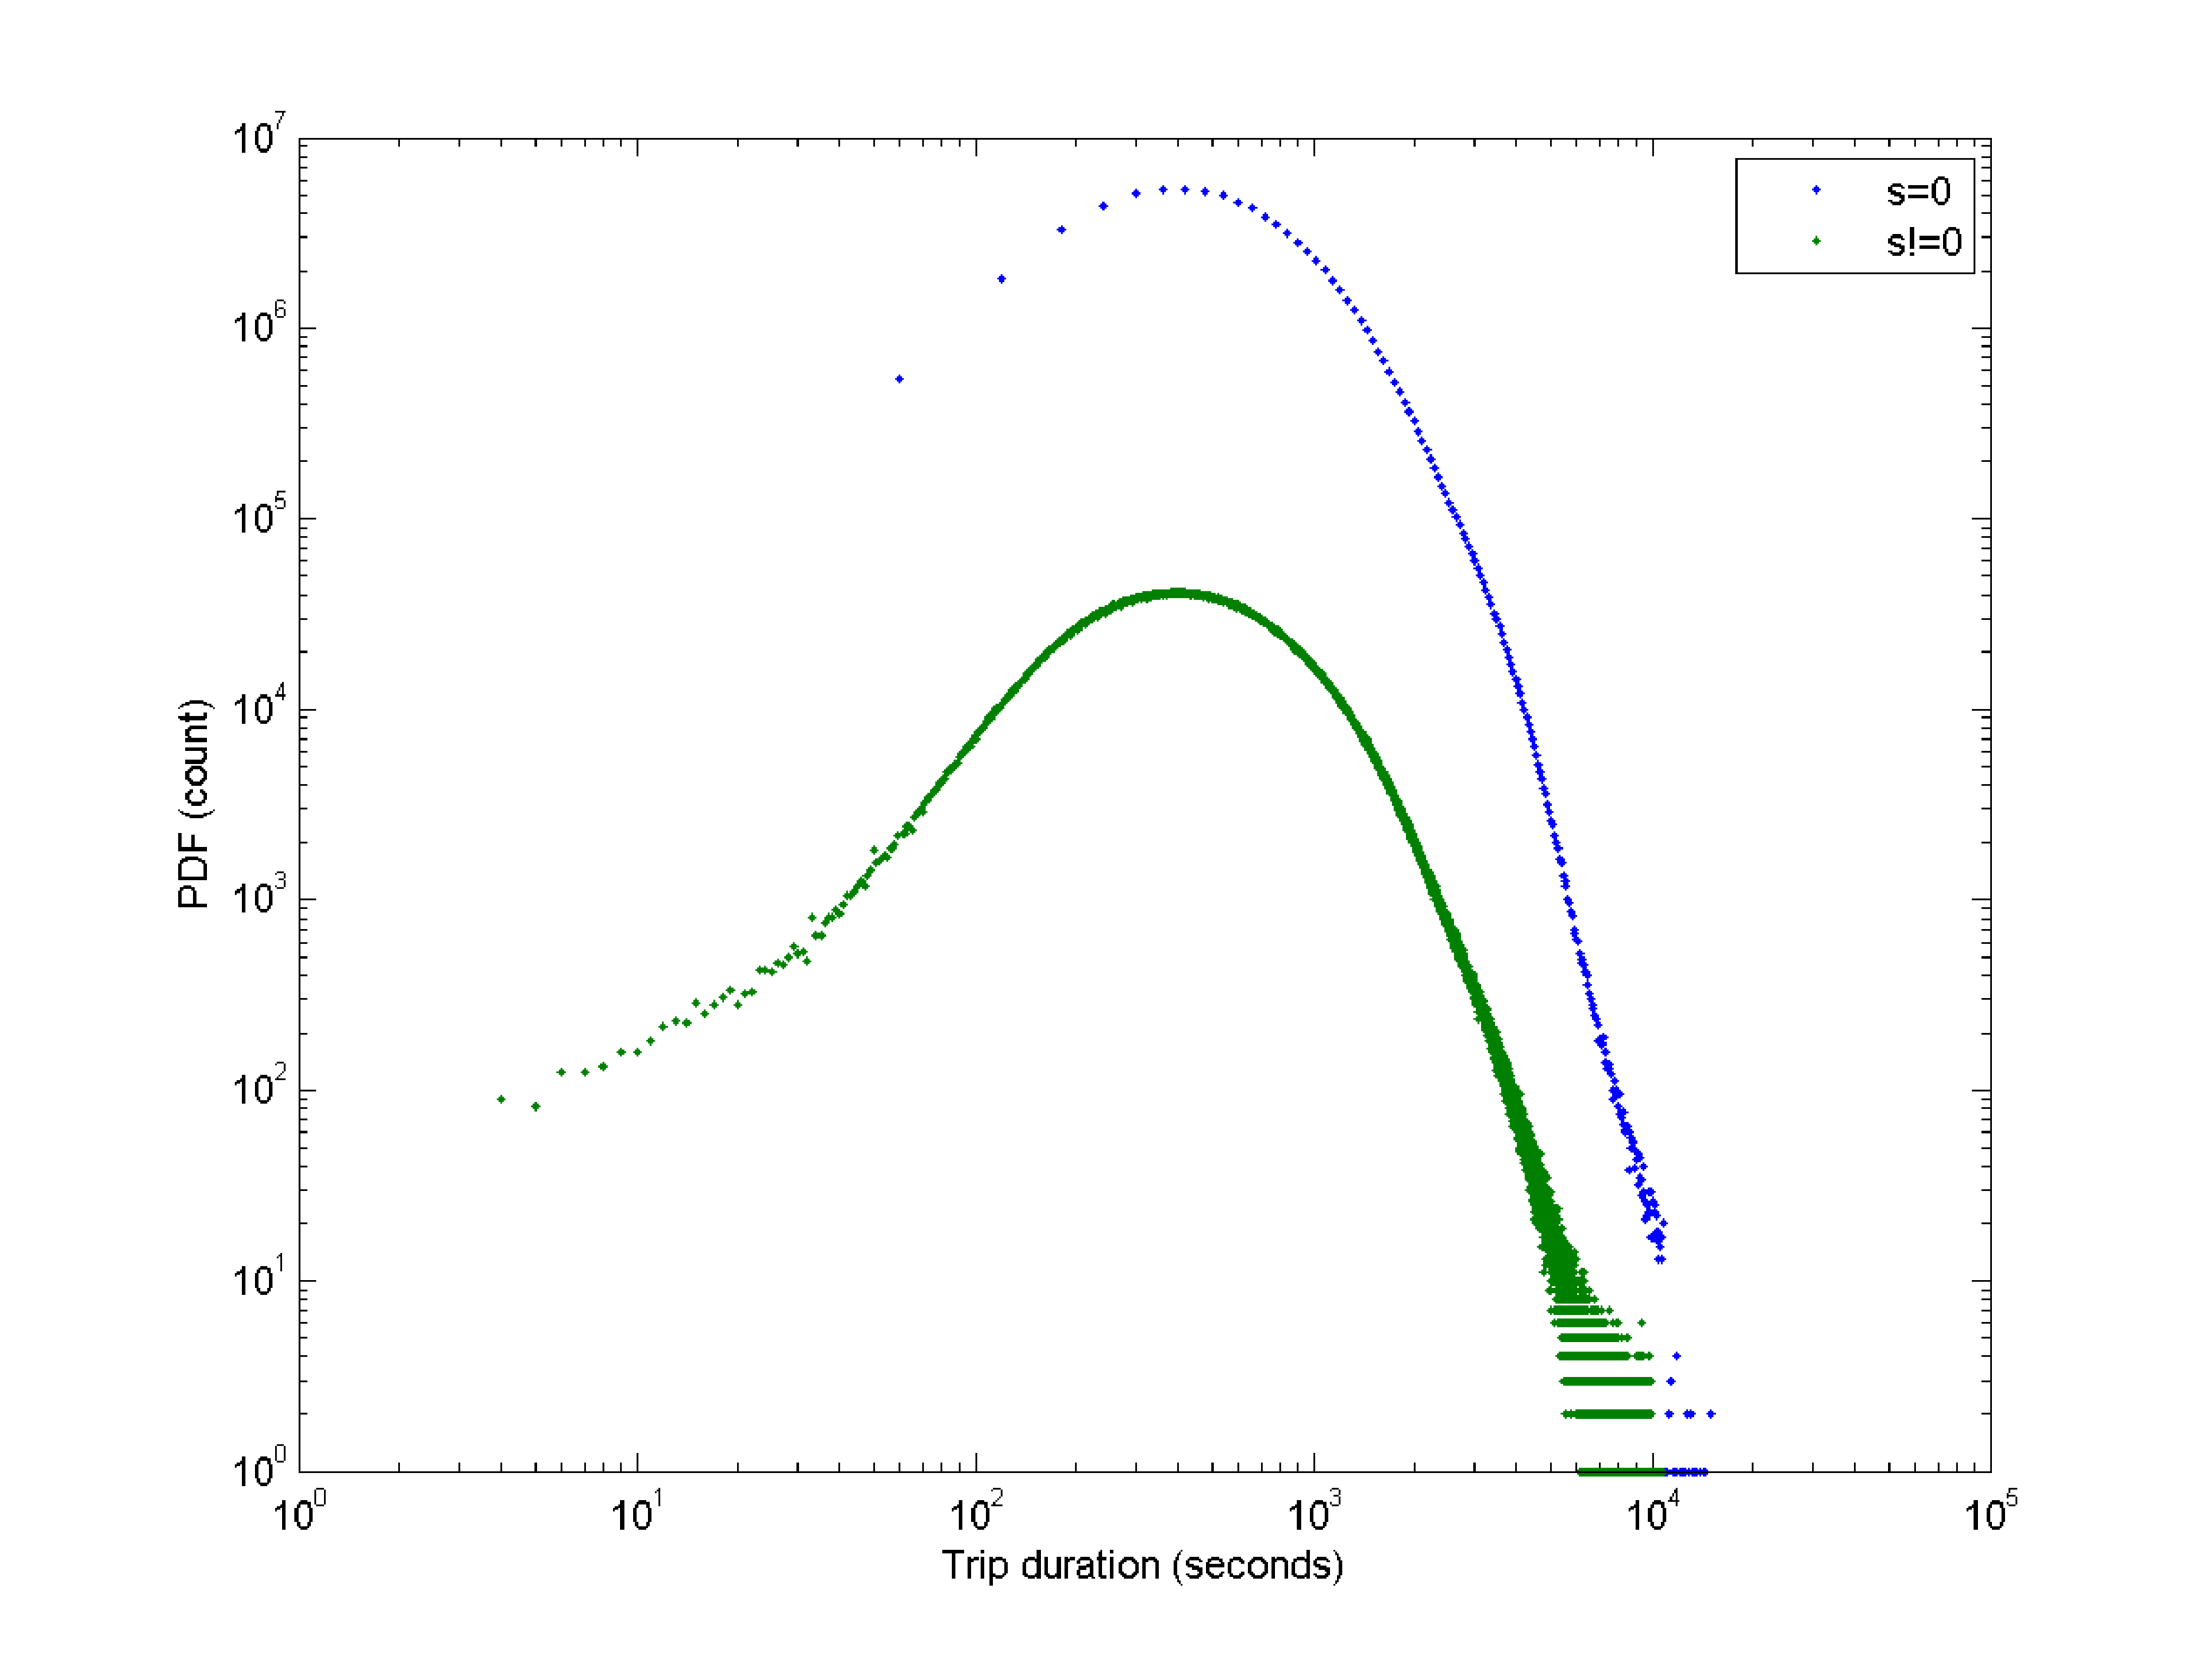
\includegraphics[scale=.20]{tpdf.eps}
\caption{Distribution of trips by time duration.}
\end{figure}

\subsection{Android Application}


The Android application was relatively straightforward.  It provides a very basic interface to the user that allows him or her to enter starting and ending coordinates for a taxi ride. To make that a little more useful in reality, there is an option to use the device's location as the starting point.  Although originally it was our intention to allow the user to enter an ending address or indicate a corner in Manhattan using two cross streets, providing that capability turns out to be a non-trivial problem.  Our map data does not have a clear mapping from nodes to street names, only latitude and longitude coordinates.  Presumably using the Google Maps API, we could translate street names into coordinates, but including that would have made for a significantly more complicated application, which we did feel was necessary in order to provide a "proof of concept."  Once the user has entered the trip coordinates, pressing a button sends these coordinates to the Amazon server as a java string.  The server parses the string and uses the data to run AStar search for distance and uses this with our model to predict time.  It then returns both of these pieces of data to the user.

Although not all of the desired features for our application have been implemented, it carries out the basic functionality that we wanted to have.  The data is sent to the server and returned with insignificant delay.

\section{Related Work}
There exist Android apps that estimate the taxi fare (such as Taxi-Calculator). However, these applications do not reveal how the fare is calculated or use the same data as our application. By focusing exclusively on New York and incorporating over ten gigabytes of taxi data into our model, we hope that our application will be able to outperform the existing applications. Additionally, by making our algorithms public, other researchers will be able to further improve the code.
Pgrouting is an open-source PostgreSQL library that supports various routing algorithms, including k-shortest-paths and A*. Additionally, pgrouting supports turn restrictions and import directly from Open Street Map data (osm2pgrouting).

Multiple websites exist that provide similar services to the one that we implemented, such as taxiwiz which calculates the fare between locations in New York City based on distance, taxi rates, and traffic levels.  TaxiFareFinder provides a service that purports to give the most accurate estimate of taxi rates.  According to its website, it uses "traffic patterns, driving speeds, urban density, and possible wait times."  The website also says that they use experimental data from users, staff, and taxi companies to improve their predictions.  Our project differed from these types of services in that we intended to use our model to check historic taxi data for systematic overcharge, as opposed to using our data only to determine an accurate prediction of a future ride.  Furthermore, our approach differs from these existing websites in terms of the data used, transparency (open-source), and machine learning techniques.  TaxiFareFinder has the advantage of a user base that can provide feedback and new data, something that would probably make predictions much more accurate\cite{taxifarefinder}.  Unfortunately, that sort of crowdsourcing source of constantly incoming data is not something we could readily access, nor was doing so the focus of our project.
\begin{figure}
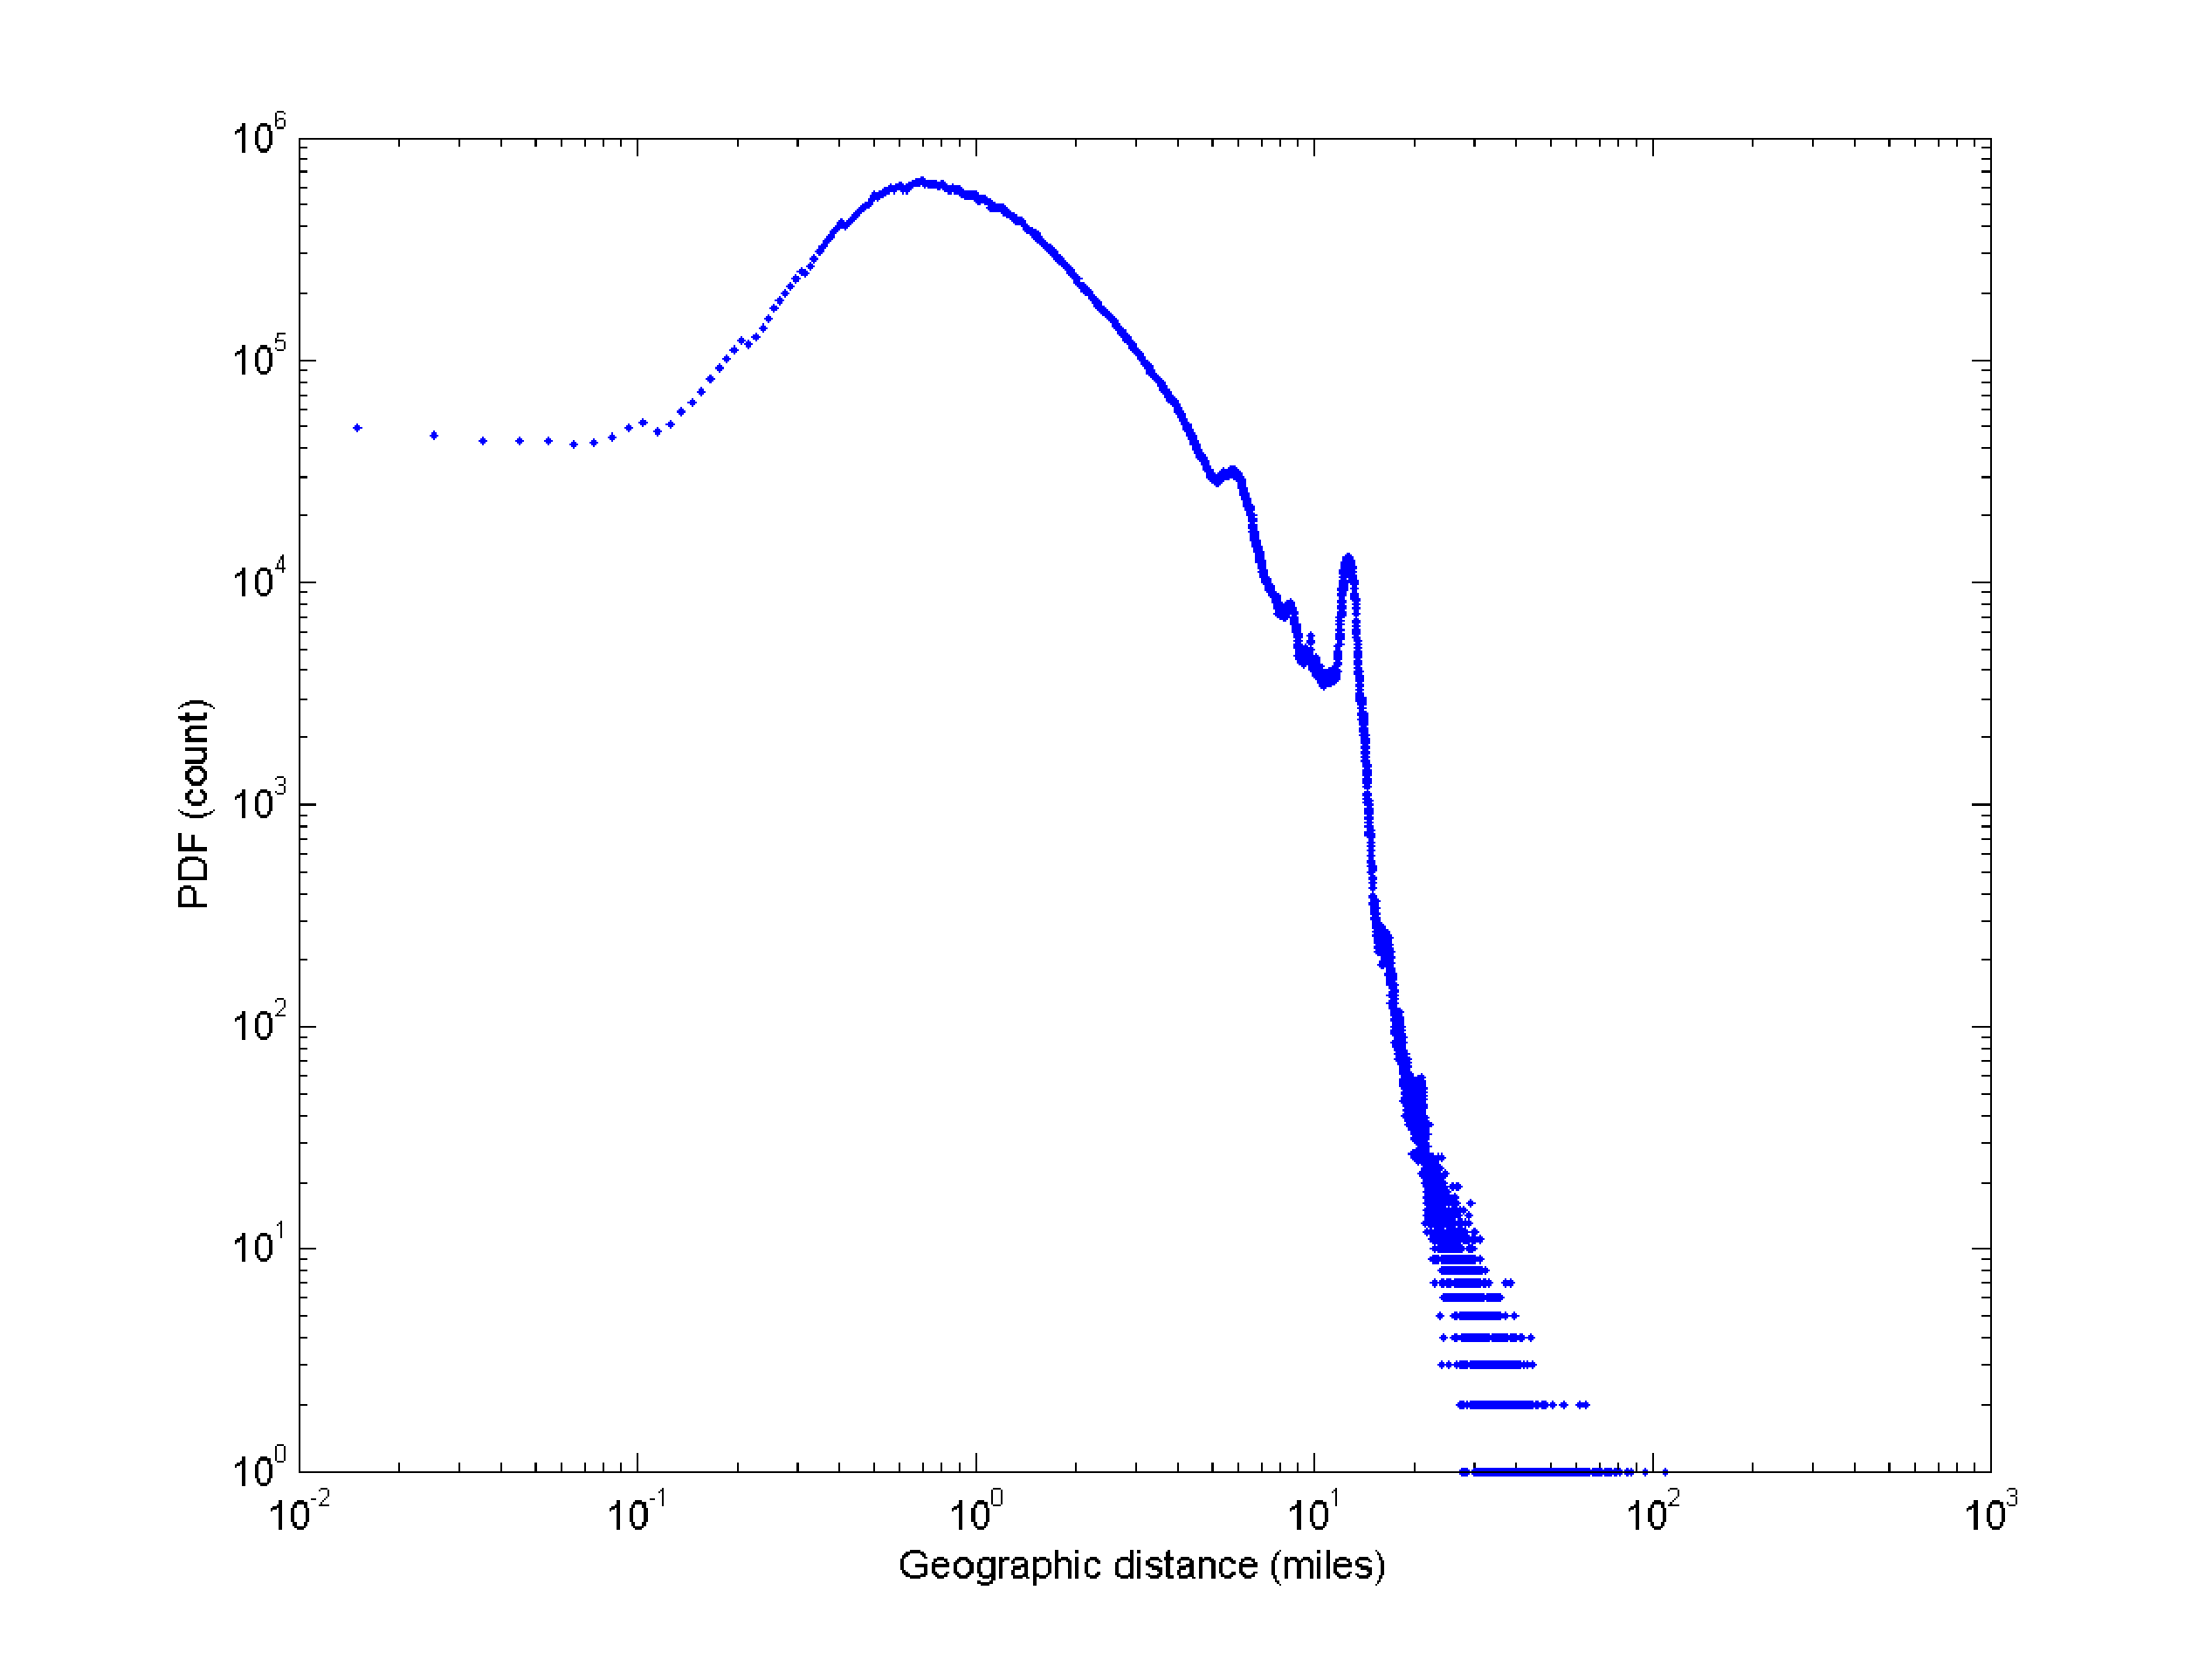
\includegraphics[scale=.19]{dpdf.eps}
\caption{Geographic distance distribution (PDF)}
\end{figure}

\begin{figure}
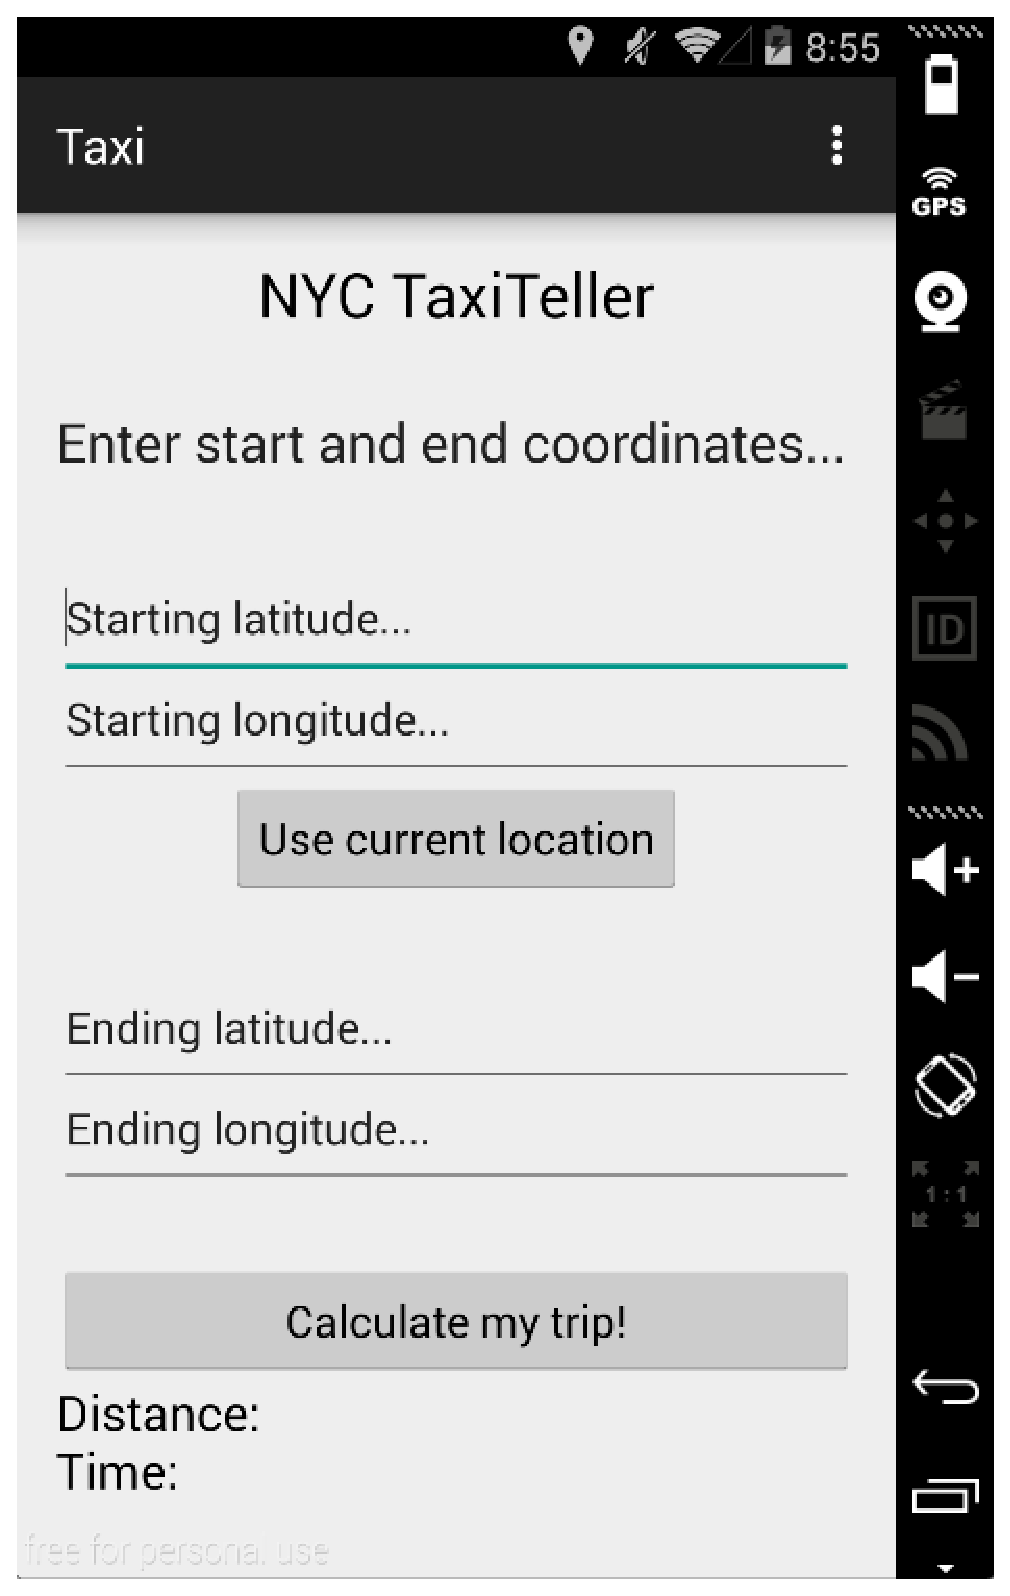
\includegraphics[scale=.30]{Screen_Shot_2015-04-16_at_3.eps}
\caption{Screenshot of Android application}
\end{figure}
\section{Conclusion}

Based on the data provided, taxi drivers tend to overcharge on quick, short trips. Taking slightly longer, perhaps waiting in more traffic to make more profit. The longer the trip is, the less a taxi driver is willing to lengthen the trip. For longer trips, based on how the cost is determined, the fare relies heavily on the distance rather than the time. Also, due to the nature of the flat start rate of \$2.50, taxi drivers during times of high traffic are incentivized to get as many trips as possible over longer or time-consuming trips.

Part of the difficulty that we faced was that our data was not as reliable or complete as we had initially hoped.  We pruned about 43.43\% of our total historic taxi data, which was around 75 million lines of data.  We had many disconnected sets in our map data.  The integrity of our data, therefore was largely suspect.  With a more reliable source, we may have had more success creating a more accurate model.  In addition, if we had access to constantly updating data or to a crowdsourcing mechanism, we would expect more accurate predictions.

Due to the nature of the data, more features would be required to have a highly accurate prediction model, however a decent model can be constructed that, save for a few large errors, generally makes a prediction to within 2-4 minutes of the actual time. In a real-world application this is generally reasonable and can serve as a good estimate for an on-the-move consumer. The data could have also been pruned to remove trips that were less than a minute in length, or less than half a mile, as issues could have arisen that caused the trip to be cut short before it even began. By pruning the data to a more normal set of distances and times, as well as pruning down to just the city, the prediction could become even more accurate.

While pruning data would be beneficial, it would be even more beneficial to get more data points. Having real-time traffic data for each street in New York City would allow us to provide a pin-point accurate prediction. While this can still vary, it would provide a better base for looking at overcharge statistics. However, the feasibility of this in practical terms is not very high and as such, close approximations are all that we can do for now.



\begin{figure}
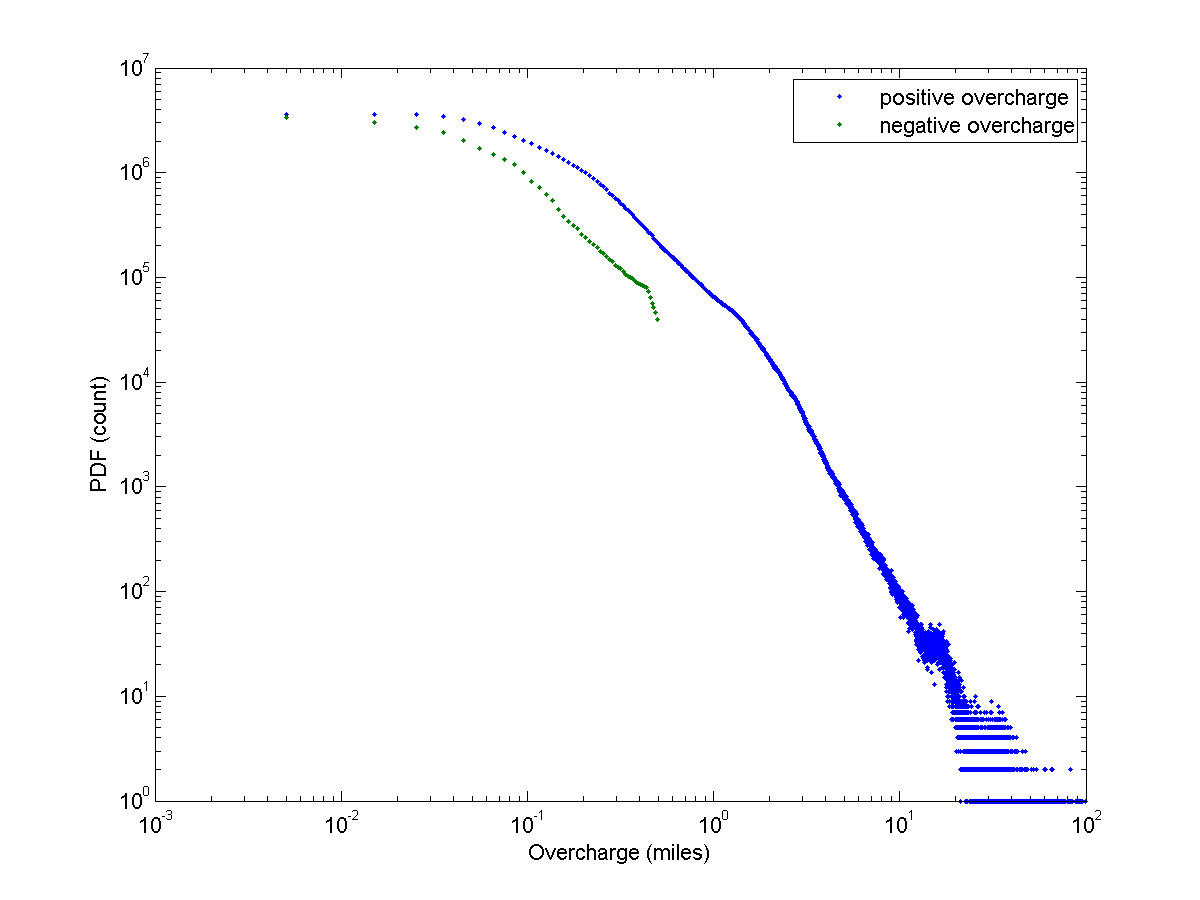
\includegraphics[scale=0.34]{opdf.eps}
\caption{Distribution of taxi trips by overcharge.}
\end{figure}

\section{Future Work}

In order to proceed with this work, we would first look to acquiring better, more accurate taxi data. A first step would be to use Freedom of Information laws to acquire the latest 2014 data. Polling the traffic-data could be useful. 

We could also create a service which end users could download to crowd-source traffic data for research purposes. With the recent introduction of Apple's research kit, creating this service for iPhone users would be fairly simple and could provide very clear data.

If we were to continue in our effort to provide a useful wrapper application to end users, there are multiple steps that would improve on our current basic design.  Any improvements to our current model would be reflected to the end user.  On top of that, it would make sense to follow the example of Taxi Fare Finder and take in user data to improve our dataset.  With any moderately sized user base, we would have data constantly coming in with which could refine our predictions.  These improvements would not be trivial, as currently our server is not set up to handle traffic from thousands of users, nor is our client side application configured in a way that makes it easily usable (currently latitude and longitude must be entered manually).  With these improvements, we could conceivably produce a useful application.  This, however, is outside the scope of our project.


\begin{figure}
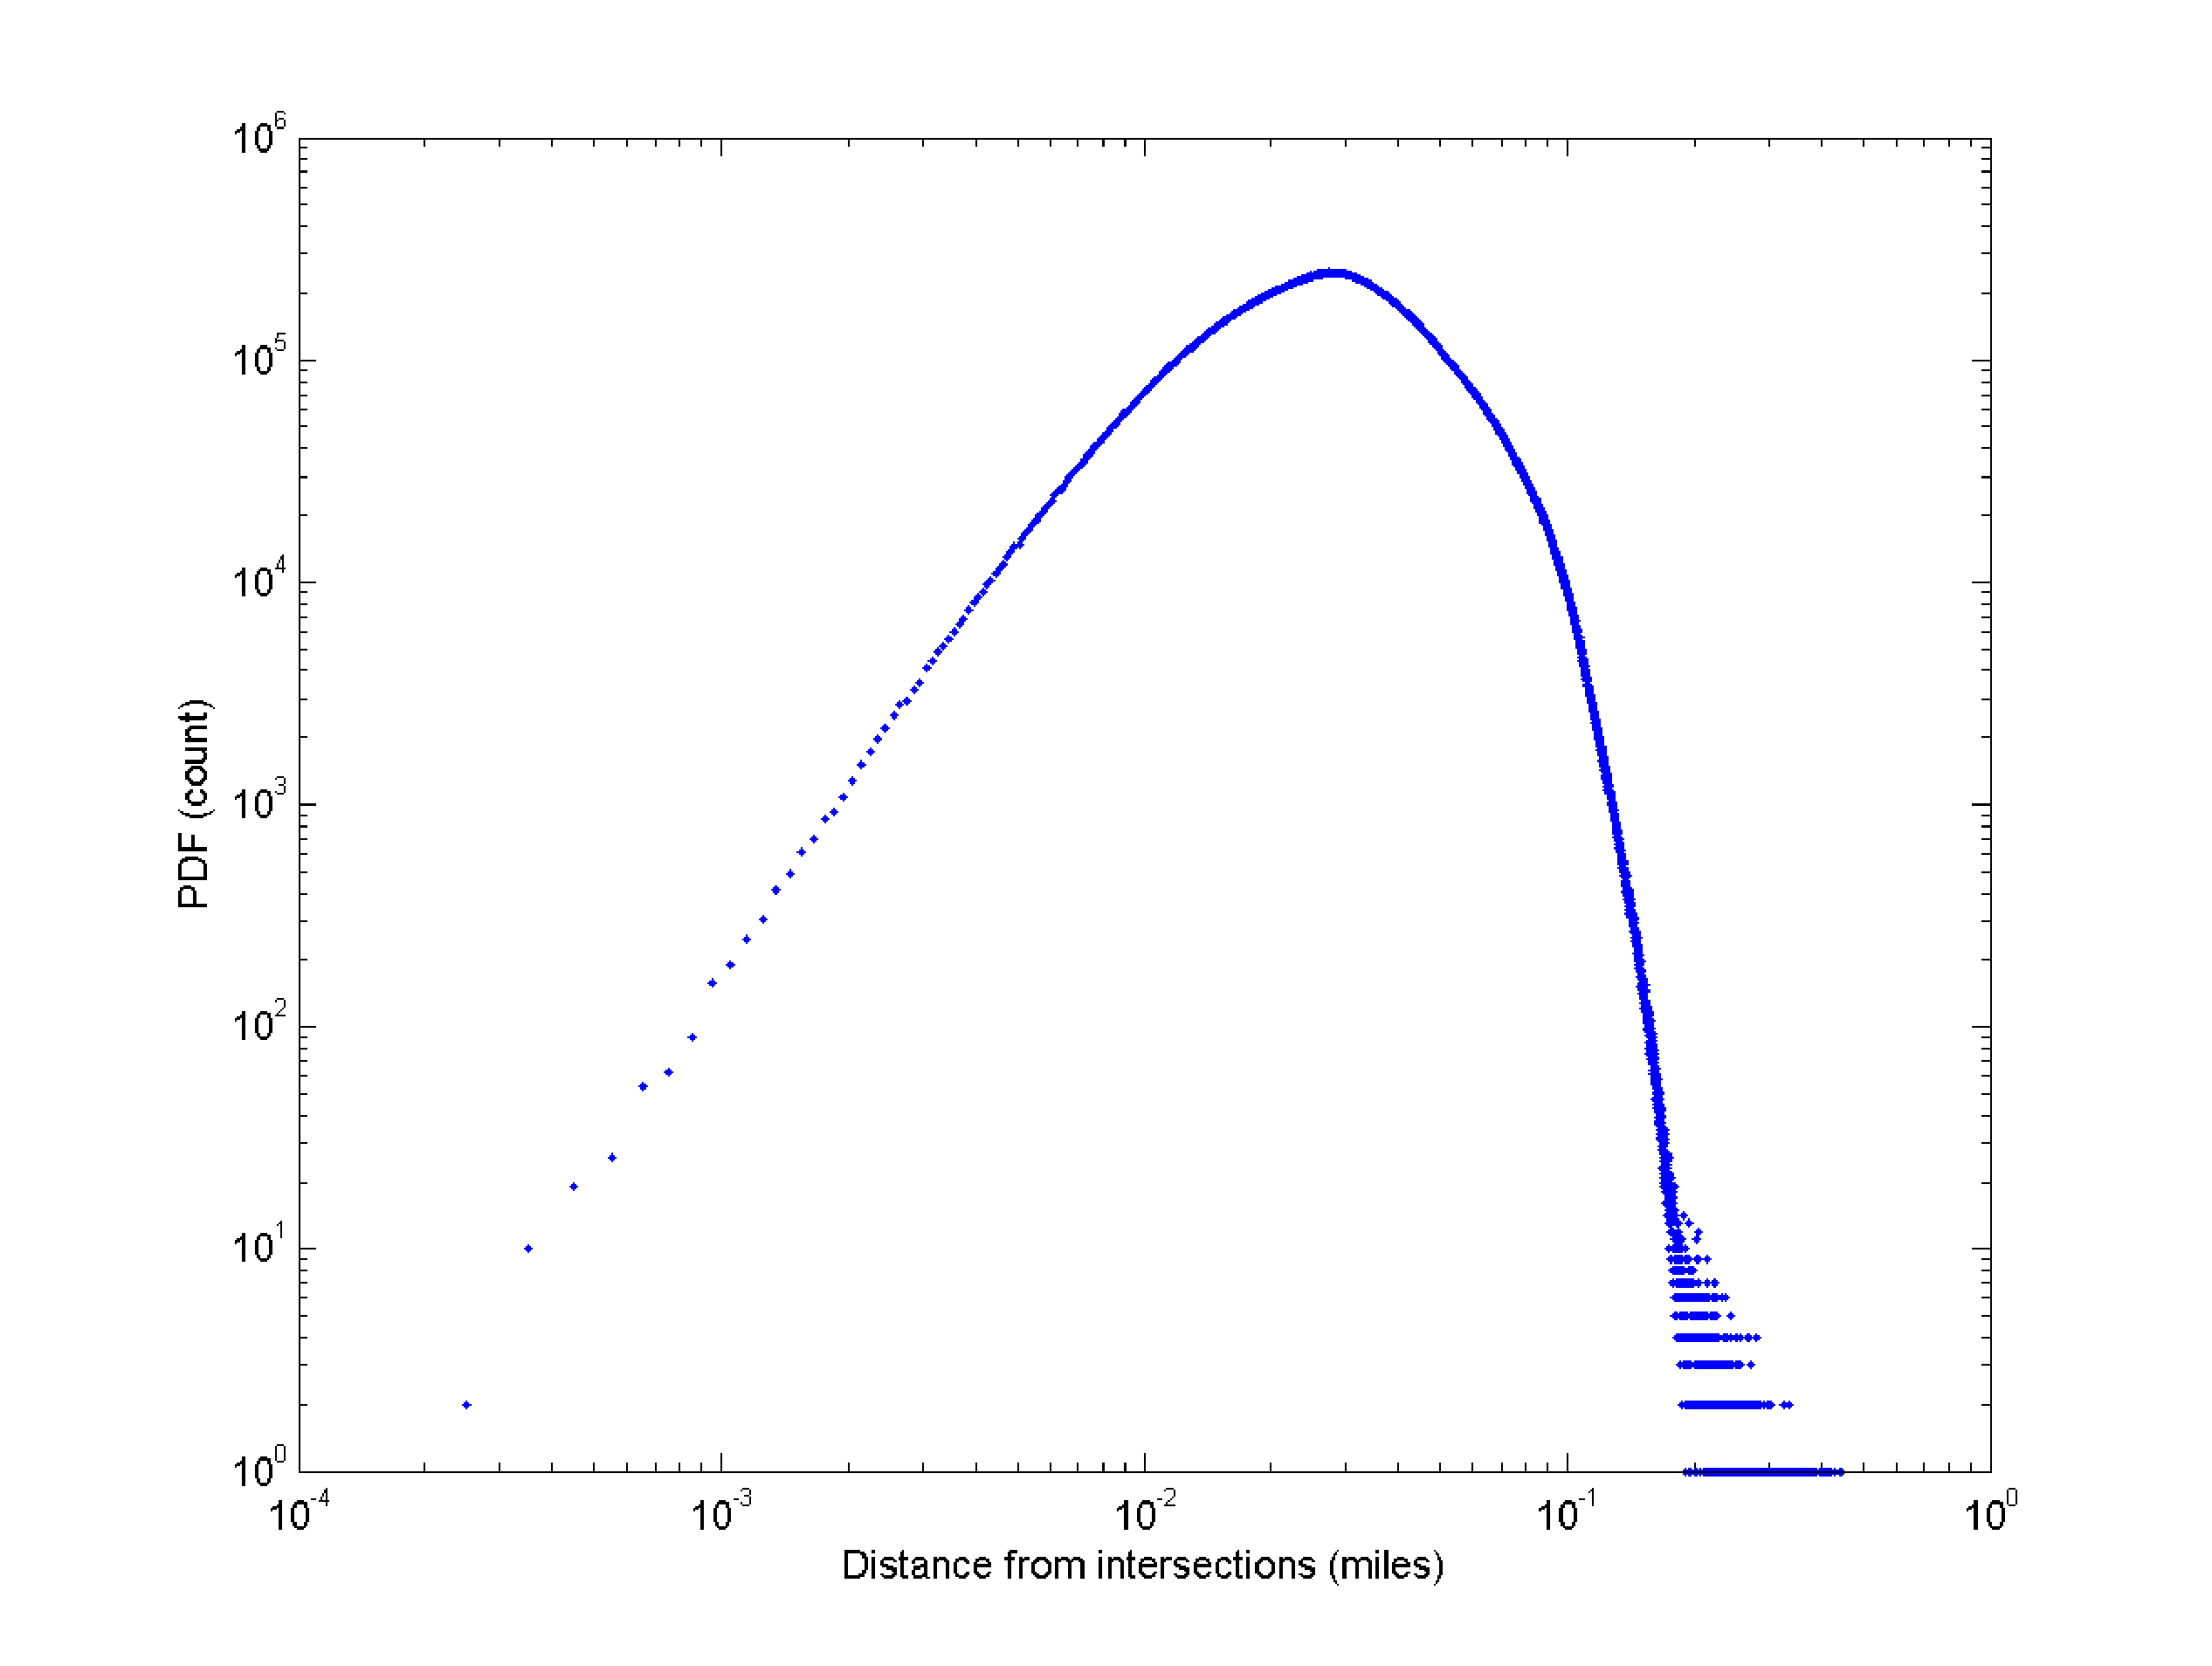
\includegraphics[scale=0.20]{epdf.eps}
\caption{Distribution of distance to start,end nodes used for the A* search. The mean distance is 0.0385 miles; the standard deviation is 0.0206 miles.}
\end{figure}

% The following two commands are all you need in the
% initial runs of your .tex file to
% produce the bibliography for the citations in your paper.
\bibliographystyle{abbrv}
\bibliography{cite.bib}
% sigproc.bib is the name of the Bibliography in this case
% You must have a proper ".bib" file
%  and remember to run:
% latex bibtex latex latex
% to resolve all references
%
% ACM needs 'a single self-contained file'!
%
%APPENDICES are optional
%\balancecolumns
%\balancecolumns % GM June 2007
% That's all folks!
\end{document}
